\documentclass[12pt,oneside,reqno]{ta-its}
\usepackage{hyperref}
\usepackage{listings}
\usepackage{float}
\usepackage{mdframed}
\usepackage{wrapfig}

\renewcommand{\lstlistingname}{Kode Sumber}
\renewcommand{\lstlistlistingname}{DAFTAR KODE SUMBER}

\title{Rancang Bangun Perangkat Lunak \textit{Internet Access Management} Berbasis Kontainer}{Design and Implementation of Internet Access Management Software Using Container}{KI141502}

\author{Fourir Akbar}{05111440000115}

\supervisorOne{Royyana Muslim Ijtihadie, S.Kom, M.Kom, PhD}{197708242006041001}
\supervisorTwo{Bagus Jati Santoso, S.Kom., Ph.D}{198611252018031001}

\degree{Sarjana Komputer}{Arsitektur dan Jaringan Komputer}{S1}{ Informatika}{Informatics}{Teknologi Informasi dan Komunikasi}{FTIK}{Information Technology and Communication}

\time{Juni}{2018}

\begin{document}
\renewcommand{\thelstlisting}{\arabic{chapter}.\arabic{lstlisting}}
	\frontmatter % Halaman dengan penomoran romawi kecil
	\maketitle
	\legalityPaper % Lembar Pengesahan
	
    \begin{abstrak}
Seiring dengan perkembangan zaman yang sangat pesat, negara-negara sudah mempunyai teknologi yang sangat maju. Teknologi mempunyai peranan yang sangat penting dalam kehidupan manusia, karena dengan adanya teknologi, manusia bisa saling berhubungan dengan mudah. Sekarang teknologi sudah semakin canggih. Teknologi yang paling populer sekarang ini adalah internet karena dengan adanya internet, banyak informasi-informasi yang dapat kita ambil dengan mudah. Internet merupakan suatu perpustakaan besar yang di dalamnya terdapat sangat banyak informasi yang berupa teks dalam bentuk media elektronik. Selain itu internet dikenal sebagai dunia maya, karena hampir seluruh aspek kehidupan di dunia nyata ada di internet, seperti olah raga, politik, hiburan, akademik, bisnis, dan lain sebagainya. Internet juga mempunyai peranan yang sangat penting dalam dunia pendidikan, karena dengan adanya internet bisa menambah ilmu pengetahuan kita dan dapat menambah motivasi belajar siswa ataupun mahasiswa. Dengan dimanfaatkan itnernet dalam dunia pendidikan agar siswa atau mahasiswa dapat memiliki komitmen untuk belajar secara aktif dan memiliki teknis kemampuan khususnya di bidang pendidikan. Oleh karena itu, internet dapat mempermudah proses belajar mengajar dengan baik.

Dalam dunia pendidikan, internet telah menjadi platform penting, misalnya adalah proses belajar mengajar yang dilakukan secara online dengan e-learning, ataupun ketika pengajar memberikan nilai kepada siswanya dilakukan secara online, dan lain sebagainya. Keamanan menjaga data-data dalam dunia pendidikan, melindungi terhadap penggunaan malware, menerapkan kepatuhan akses internet, menyederhanakan manajemen jaringan menjadi tantangan utama untuk manajemen TI. Maka dari itu dibutuhkan sebuah server yang digunakan sebagai internet access management atau untuk melakukan manajemen akses terhadap user yang menggunakan jaringannya.

Namun akan terjadi permasalahan ketika banyak user yang mengakses internet dengan menggunakan server yang digunakan sebagai internet access management. Dalam pembacaan log history dari setiap user akan tercampur karena hanya melewati satu server saja. 

Dalam tugas akhir ini akan dibuat sebuah rancangan sistem pada server yang akan dijadikan sebagai internet access management, yang memungkinkan untuk mencatat setiap log history dari setiap user yang mengakses internet secara detail. Rancangan sistem pada server akan menggunakan kontainer docker. Kontainer docker merupakan operating-system-level virtualization untuk menjalankan beberapa sistem linux yang terisolasi (kontainer) pada sebuah host. Kontainer berfungsi untuk mengisolasi aplikasi atau servis dan dependensinya. Untuk setiap servis atau aplikasi yang terisolasi dibutuhkan satu kontainer pada server host yang ada dan setiap kontainer akan menggunakan sumber daya yang ada pada server host selama kontainer tersebut menyala.\\

	\noindent \textbf{Kata-Kunci}: Docker, Internet Access Management, Kontainer
\end{abstrak}
\newpage
\begin{abstract}
Along with the rapid development of the era, the countries already have advanced technology. Technology has a very important role in human life, because with technology, humans can interconnect easily. Now, technology is getting more sophisticated. The most popular technology today is internet, because with  internet, we can take a lot of information easily. Internet is one of the very many media information that contains text in the form of electronic media. In addition, internet is known as virtual word, because various aspects of life in the world, such as sports, politics, entertainment, educations, business, etc. Internet also has a very important role in the world of education, because internet can increase our knowledge and can increase students motivation to learn. Therefor, internet can help learning process well.

Internet has become a vital platform for most educations, for example is the process of teaching and learning that is done oneline with e-learning, or when teachers / lecturers provide score to their students are done online, etc. Safe guarding data, protecting against malware usages, implementing internet access compliance, simplifying network management become the key challenges for IT management. Therefore required a server that is used as internet access management or to perform management access to users who use the network.

But there will be problems when many users who access internet by using a server that is used as internet access management. In reading log history of each user will be mixed because only through one server only.

In this final project will be created a system design on the server that will serve as internet access management, which allows to record every log history of each user who access internet in detail. The system design on the server will user docker containers. Docker containers is an operating system level virtualization to run some isolated linux systems (containers) on a host. Containers are used to isolate applications or services and its dependencies. For every service or app that isolated it takes one container on the existing host server and each container will user the existing resources on the host server as long as the container is on.\\

	\noindent \textbf{Keywords}: Container, Docker, Internet Access Management
\end{abstract}
	\chapter{Kata Pengantar}
		\begin{figure}[h]
			\centering
			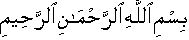
\includegraphics[width=0.5\linewidth]{img/bismillah.png}
		\end{figure}

		Alhamdulillahirabbil’alamin, segala puji bagi Allah SWT, yang telah melimpahkan rahmat dan hidayah-Nya sehingga penulis dapat menyelesaikan Tugas Akhir yang berjudul \textbf{Rancang Bangun Perangkat Lunak Internet \textit{Acces Management} Berbasis Kontainer}. Pengerjaan Tugas Akhir ini merupakan suatu kesempatan yang sangat baik bagi penulis. Dengan pengerjaan Tugas Akhir ini, penulis bisa belajar lebih banyak untuk memperdalam dan meningkatkan apa yang telah didapatkan penulis selama menempuh perkuliahan di Teknik Informatika ITS. Dengan Tugas Akhir ini penulis juga dapat menghasilkan suatu implementasi dari apa yang telah penulis pelajari.
		Selesainya Tugas Akhir ini tidak lepas dari bantuan dan dukungan beberapa pihak. Sehingga pada kesempatan ini penulis mengucapkan syukur dan terima kasih kepada:
		\begin{enumerate}
			\item Allah SWT atas anugerahnya yang tidak terkira kepada penulis dan Nabi Muhammad SAW.
			\item Bapak, Mama, dan keluarga Penulis yang selalu memberikan perhatian, dorongan dan kasih sayang yang menjadi semangat utama bagi diri Penulis sendiri baik selama penulis menempuh masa perkuliahan maupun pengerjaan Tugas Akhir ini.
			\item Bapak Royyana Muslim Ijtihadie, S.Kom., M.Kom., PhD. selaku Dosen Pembimbing yang telah banyak meluangkan waktu untuk memberikan ilmu, nasihat, motivasi, pandangan dan bimbingan kepada Penulis baik selama Penulis menempuh masa kuliah maupun selama pengerjaan Tugas Akhir ini.
			\item Bagus Jati Santoso, S.Kom., PhD. selaku dosen pembimbing yang telah memberikan ilmu, dan masukan kepada Penulis.
			\item Seluruh tenaga pengajar dan karyawan Jurusan Teknik Informatika ITS yang telah memberikan ilmu dan waktunya demi berlangsungnya kegiatan belajar mengajar di Jurusan Teknik Informatika ITS.
			\item Seluruh teman Penulis di Jurusan Teknik Informatika ITS yang telah memberikan dukungan dan semangat kepada Penulis selama Penulis menyelesaikan Tugas Akhir ini.
			\item Teman-teman, Kakak-kakak dan Adik-adik \textit{administrator} Laboratorium Arsitektur dan Jaringan Komputer yang selalu menjadi teman untuk berbagi ilmu.
		\end{enumerate}

		Penulis menyadari bahwa Tugas Akhir ini masih memiliki banyak kekurangan. Sehingga dengan kerendahan hati, penulis mengharapkan kritik dan saran dari pembaca untuk perbaikan ke depannya.

		\hfill Surabaya, Juni 2018 \\ \\
		\hfill Fourir Akbar

	\cleardoublepage % Mengisi penanda halaman genap yang kosong

	\tableofcontents % Daftar Isi
	\listoftables % Daftar Tabel
	\listoffigures % Daftar Gambar
	\lstlistoflistings % Daftar Kode Sumber

	\mainmatter
	\chapter{PENDAHULUAN}
Pada bab ini akan dipaparkan mengenai garis besar Tugas Akhir yang meliputi latar belakang, tujuan, rumusan dan batasan permasalahan, metodologi pembuatan Tugas Akhir, dan sistematika penulisan.

\section{Latar Belakang}
Seiring dengan perkembangan zaman yang sangat pesat, negara-negara sudah mempunyai teknologi yang sangat maju. Teknologi mempunyai peranan yang sangat penting dalam kehidupan manusia, karena dengan adanya teknologi, manusia bisa saling berhubungan dengan mudah. Sekarang teknologi sudah semakin canggih. Teknologi yang paling populer sekarang ini adalah internet karena dengan adanya internet, banyak informasi-informasi yang dapat kita ambil dengan mudah. Internet merupakan suatu perpustakaan besar yang di dalamnya terdapat sangat banyak informasi yang berupa teks dalam bentuk media elektronik. Selain itu internet dikenal sebagai dunia maya, karena hampir seluruh aspek kehidupan di dunia nyata ada di internet, seperti olah raga, politik, hiburan, akademik, bisnis, dan lain sebagainya. Internet juga mempunyai peranan yang sangat penting dalam dunia pendidikan, karena dengan adanya internet bisa menambah ilmu pengetahuan kita dan dapat menambah motivasi belajar siswa ataupun mahasiswa. Dengan dimanfaatkan internet dalam dunia pendidikan agar siswa atau mahasiswa dapat memiliki komitmen untuk belajar secara aktif dan memiliki teknis kemampuan khususnya di bidang pendidikan. Oleh karena itu, internet dapat mempermudah proses belajar mengajar dengan baik.

Dalam dunia pendidikan, internet telah menjadi \textit{platform} penting, misalnya adalah proses belajar mengajar yang dilakukan secara \textit{online} dengan e-learning, ataupun ketika pengajar memberikan nilai kepada siswanya dilakukan secara \textit{online}, dan lain sebagainya. Keamanan menjaga data-data dalam dunia pendidikan, melindungi terhadap penggunaan malware, menerapkan kepatuhan akses internet, menyederhanakan manajemen jaringan menjadi tantangan utama untuk manajemen TI. Maka dari itu dibutuhkan sebuah \textit{online} yang digunakan sebagai \textit{internet access management} atau untuk melakukan manajemen akses terhadap \textit{user} yang menggunakan jaringannya.

Namun akan terjadi permasalahan ketika banyak \textit{user} yang mengakses internet dengan menggunakan \textit{server} yang digunakan sebagai \textit{internet access management}. Dalam pembacaan \textit{log history} dari setiap \textit{user} akan tercampur karena hanya melewati satu \textit{server} saja. 

Dalam tugas akhir ini akan dibuat sebuah rancangan sistem pada \textit{server} yang akan dijadikan sebagai \textit{internet access management}, yang memungkinkan untuk mencatat setiap \textit{log history} dari setiap \textit{user} yang mengakses internet secara detail. Rancangan sistem pada \textit{server} akan menggunakan kontainer \textit{docker}. Kontainer \textit{docker} merupakan \textit{operating-system-level virtualization} untuk menjalankan beberapa sistem linux yang terisolasi (kontainer) pada sebuah host. Kontainer berfungsi untuk mengisolasi aplikasi atau servis dan dependensinya. Untuk setiap servis atau aplikasi yang terisolasi dibutuhkan satu kontainer pada \textit{server host} yang ada dan setiap kontainer akan menggunakan sumber daya yang ada pada \textit{server host} selama kontainer tersebut menyala.

\section{Rumusan Masalah}
Berikut beberapa hal yang menjadi rumusan masalah dalam tugas akhir ini:
\begin{enumerate}
	\item Bagaimana cara \textit{client} untuk melakukan \textit{autentifikasi}?
	\item Bagaimana cara membuat sebuah kontainer \textit{docker} secara otomatis ketika terdapat \textit{client} yang akan mengakses internet?
	\item Bagaimana cara mengarahkan \textit{traffic} dari \textit{client} ke kontainer \textit{docker} yang sesuai?
	\item Bagaimana cara mencatat aktivitas dari \textit{client}?
	\item Bagaimana perbandingan performa antara IAM konvensional dengan IAM berbasi kontainer?
	\item Bagaimana mengevaluasi penggunaan sumber daya dan skalabilitas pada \textit{docker host}?
\end{enumerate}

\section{Batasan Masalah}
Dari permasalahan yang telah diuraikan di atas, terdapat beberapa batasan masalah pada tugas akhir ini, yaitu:
\begin{enumerate}
	\item Satu \textit{client} yang berhasil \textit{login} akan disediakan satu kontainer.
	\item Kontainer yang digunakan adalah \textit{docker}.
	\item Parameter untuk mengetahui apa saja yang diakses oleh \textit{client} adalah \textit{access log} dari \textit{client} tersebut.
	\item Setiap \textit{client} mendapatkan IP \textit{private}.
	\item Performa yang diukur adalah \textit{response time}.
	\item Bahasa pemrograman yang digunakan adalah \textit{Python}.
\end{enumerate}

\section{Tujuan}
Tugas akhir dibuat dengan beberapa tujuan. Berikut beberapa tujuan dari pembuatan tugas akhir:
\begin{enumerate}
	\item Mengetahui cara bagaimana \textit{client} dapat melakukan \textit{autentifikasi}.
	\item Mengimplementasikan metode untuk membuat sebuah kontainer terhadap \textit{client} yang telah berhasil \textit{login} ke jaringan ITS.
	\item Mengetahui cara untuk mengarahkan \textit{traffic} dari \textit{client} ke kontainer \textit{docker} yang sesuai.
	\item Mengetahui bagaimana cara mencatat aktivitas \textit{client}.
	\item Mengetahui bagaimana perbandingan performa antara IAM konvensional dengan IAM berbasis kontainer.
	\item Mengetahui penggunaan sumber daya dan skalabilitas pada \textit{docker host}.
\end{enumerate}

\section{Manfaat}
Tugas akhir dibuat dengan beberapa manfaat. Berikut beberapa manfaat dari pembuatan tugas akhir:
\begin{enumerate}
	\item Mengetahui cara bagaimana \textit{client} dapat melakukan \textit{autentifikasi}.
	\item Mengethaui cara untuk mengarahkan \textit{traffic} dari \textit{client} ke kontainer \textit{docker} yang sesuai.
	\item Mempermudah pencatatan aktivitas dari masing-masing \textit{client} yang mengakses internet.
	\item Meringankan beban dari penggunaan \textit{server} di ITS karena penggunaan kontainer \textit{docker} lebih ringan.
\end{enumerate}      

\section{Metodologi}
Metodologi yang digunakan pada pengerjaan Tugas Akhir ini
adalah sebagai berikut:
\subsection{Studi literatur}
Studi literatur merupakan langkah yang dilakukan untuk mendukung dan memastikan setiap tahap pengerjaan tugas akhir sesuai dengan standar dan konsep yang berlaku. Pada tahap studi literatur ini, akan dilakukan studi mendalam mengenai kontainer \textit{docker}, \textit{flask}, \textit{mitmproxy}, dan pembuatan aturan dengan menggunakan \textit{iptables}. Adapun literatur yang dijadikan sumber berasal dari paper, buku, materi perkuliahan, forum serta artikel dari internet.

\subsection{Desain dan Perancangan Sistem}
Tahap ini meliputi perancangan sistem berdasarkan studi literatur dan pembelajaran konsep. Tahap ini merupakan tahap yang paling penting dimana bentuk awal aplikasi yang akan diimplementasikan didefinisikan. Pada tahapan ini dibuat kasus penggunaan yang ada pada sistem, arsitektur sistem, serta perencanaan implementasi pada sistem.
\subsection{Implementasi Sistem}
Implementasi merupakan tahap membangun implementasi rancangan sistem yang telah dibuat. Pada tahapan ini merealisasikan apa yang telah didesain dan dirancang pada tahapan sebelumnya, sehingga menjadi sebuah sistem yang sesuai dengan apa yang telah direncanakan.
\subsection{Uji Coba dan Evaluasi}
Pada tahapan ini dilakukan uji coba terhadap sistem yang telah dibuat. Pengujian dan evaluasi akan dilakukan dengan melihat kesesuaian dengan perencanaan. Selain itu, tahap ini juga akan melakukan uji performa sistem dan melakukan perbandingan dengan metode lain untuk mengetahui efisiensi penggunaan sumber daya serta evaluasi berdasarkan hasil uji performa tersebut. 

\section{Sistematika Laporan}
Buku tugas akhir ini bertujuan untuk mendapatkan gambaran dari pengerjaan tugas akhir ini. Selain itu, diharapkan dapat berguna bagi pembaca yang berminat melakukan pengambangan lebih lanjut. Secara garis besar, buku tugas akhir ini terdiri atas beberapa bagian seperti berikut:
\begin{enumerate}
	
	\item \textbf{Bab I} \indent \textbf{Pendahuluan} \\        
	\indent \indent Bab yang berisi latar belakang, tujuan, manfaat, permasalahan, batasan masalah, metodologi yang digunakan dan sistematika laporan.
	\\
	\item \textbf{Bab II} \indent \textbf{Dasar Teori}
	\\
	\indent \indent Bab ini berisi penjelasan secara detail mengenai dasar-dasar penunjang dan teori-teori yang yang digunakan dalam pembuatan tugas akhir ini.
	\\
	\item \textbf{Bab III} \indent \textbf{Desain dan Perancangan}
	\\
	\indent \indent Bab ini berisi tentang analisis dan perancangan sistem yang dibuat, termasuk di dalamnya mengenai analisis kasus penggunaan, desain arsitektur sistem, dan perancangan implementasi sistem.
	\\
	\item \textbf{Bab IV} \indent \textbf{Implementasi}
	\\
	\indent \indent Bab ini membahas implementasi dari desain yang telah dibuat pada bab sebelumnya. Penjelasan berupa pemasangan alat dan kode program yang digunakan untuk mengimplementasikan sistem.
	\\
	\item \textbf{Bab V} \indent \textbf{Uji Coba dan Evaluasi}
	\\
	\indent \indent Bab ini membahas tahap-tahap uji coba serta melakukan evaluasi terhadap sistem yang dibuat.
	\\
	\item \textbf{Bab VI} \indent \textbf{Kesimpulan dan Saran}
	\\
	\indent \indent Bab ini merupakan bab terakhir yang memberikan kesimpulan dari hasil percobaan dan evaluasi yang telah dilakukan. Pada bab ini juga terdapat saran bagi pembaca yang berminat untuk melakukan pengembangan lebih lanjut.    
\end{enumerate}
	\chapter{TINJAUAN PUSTAKA}
\section{Python}
Python adalah bahasa pemrograman interpretatif multiguna dengan prinsip agar sumber kode yang dihasilkan memiliki tingkat keterbacaan yang baik. Python diklaim sebagai bahasa yang menggabungkan kapabilitas, kemampuan, dengan sintaksis kode yang sangat jelas, dan dilengkapi dengan fungsionalitas pustaka standar yang besar serta komprehensif. Python mendukung beragam paradigma pemrograman, seperti pemrograman berorientasi objek, pemrograman imperatif, dan pemrograman fungsional. Python dapat digunakan untuk berbagai keperluan pengembangan perangkat lunak dan dapat berjalan di berbagai platform sistem operasi. \cite{bab2-python} \\

\section{Flask}
Flask adalah sebuah kerangka kerja web. Artinya, Flask menyediakan perangkat, pustaka, dan teknologi yang memungkinkan seorang pengembang untuk membangun aplikasi berbasis web. Aplikasi web yang bisa dibangun bisa berupa sebuah halaman web, blog, wiki, bahkan untuk web komersial. Flask dibangun berbasiskan pada Werkzeug, Jinja 2, dan MarkupSafe yang mana menggunakan bahasa pemrograman Python sebagai basisnya. Flask sendiri pertama kali dikembangkan pada tahun 2010 dan didistribusikan dengan lisensi BSD. \cite{bab2-flask} \\
\indent Flask termasuk sebagai perangkat kerja mikro karena tidak membutuhkan banyak perangkat atau pustaka tertentu agar bisa bekerja. Flask tidak menyediakan fungsi untuk melakukan interaksi dengan basis data, tidak mempunya validasi \textit{form} atau fungsi lain yang umumnya bisa digunakan dan disediakan pada sebuah kerangka kerja web. Meskipun memiliki kemampuan yang minim, tapi Flask mendukung dan memberikan kemudahan bagi pengembang untuk menambahkan pustaka sendiri untuk mendukung aplikasinya. Berbagai pustaka seperti validasi \textit{form}, mengunggah file, berbagai macam teknologi autentifikasi bisa digunakan dan tersedia untuk Flask. Bahkan pustaka-pustaka pendukung tersebut lebih sering diperbarui dibandingkan dengan Flasknya sendiri.

\section{Gunicorn}
Gunicorn atau '\textit{Green Unicorn}' adalah {Python} WSGI HTTP \textit{Server} untuk UNIX. Fungsi dari \textit{Gunicorn} ini adalah sebagai pelayan sebuah aplikasi atau sebagai server dari sebuah perangkat lunak yang dikembangkan oleh pengembang.

\textit{Gunicorn} sendiri merupakan salah satu dari sekian banyak \textit{WSGI Server}. Keunggulan dari \textit{Gunicorn} sendiri adalah, \textit{Gunicorn} mampu menangani atau kompatibel dengan berbagai macam kerangka kerja web, sangat mudah untuk diimplementasikan, hanya membutuhkan sedikit sumber daya dari \textit{server} yang terpasang \textit{Gunicorn}, dan juga kerja dari \textit{Gunicorn} yang sangat cepat.

\textit{Gunicorn} mengimplementasikan spesifikasi standar \textit{server WSGI PEP3333} sehingga dapat menjalankan perangkat lunak berbasis \textit{web} yang dikembangkan dengan bahasa pemrograman \textit{python}. Sebagai contoh, perangkat lunak berbasis web yang digunakan oleh penulis menggunakan kerangka kerja \textit{flask}, maka \textit{Gunicorn} dapat menanganinya.

\section{\textit{Supervisor}}
\textit{Supervisor} adalah sistem yang berbasis \textit{client} atau server, yang memungkinkan penggunanya utuk memantau dan juga mengontrol sejumlah proses pada sistem operasi untuk UNIX. Beberapa faktor terbentuknya \textit{supervisor} antara lain adalah, kenyamanan, ketepatan, delegasi, dan proses grup dalam menggunakan perangkat lunak \textit{supervisor}. Beberapa keunggulan dari perangkat lunak \textit{supervisor} antara lain, konfigurasi yang sederhana, proses yang terpusat, efisien, dapat diperluas penggunaannya, dan juga kompatibel dengan berbagai macam sistem operasi. Komponen dari \textit{supervisor} terbagi menjadi dua, antara lain sebagai berikut.

\subsection{\textit{Supervisord}}
\textit{Supervisord} merupakan bagian dari \textit{supervisor} yang bertanggung jawab untuk memulai \textit{child programs} atas permintaannya sendiri, menanggapi perintah dari \textit{client}, melakukan \textit{restart} secara otomatis ketika terjadi kerusakan pada proses, mencatat bagian dari proses \texttt{stdout} dan \texttt{stderr} \textit{output}, juga menghasilan dan menangani \textit{events} yang berhubungan dengan bagian-bagian yang digunakan selama \textit{subprocess} tersebut berjalan.

\subsection{\textit{Supervisorctl}}
\textit{Supervisorctl} merupakan bagian dari \textit{command-line} yang digunakan oleh \textit{client}. \textit{Supervisorctl} menyediakan antarmuka yang mirip dengan fitur \textit{shell} yang disediakan oleh \textit{supervisord}. Dari \textit{supervisorctl}, pengguna dapat terhubung dengan proses \textit{supervisord} yang berbeda satu per satu, mendapatkan status dari \textit{subprocess} yang telah dikontrol, menghentikan atau memulai \textit{subprocess} yang telah dikontrol, dan juga mendapatkan semua daftar proses yang berjalan pada \textit{supervisord}.

\textit{Command-line} dari \textit{client} berhubungan ke \textit{server} melalui \textit{socket domain} UNIX atau melalui \textit{socker internet} (TCP). \textit{Server} dapat menyatakan bahwa \textit{client} harus memberikan \textit{autentifikasi} sebelum mengizinkannya untuk melakukan sebuah perintah. Proses \textit{client} biasanya menggunakan \textit{file} konfigurasi yang sama dengan \textit{server}. 

\section{\textit{Nginx}}
Nginx adalah sebuah perangkat lunak yang bisa digunakan untuk \textit{web server}, \textit{load balancer}, dan \textit{reverse proxy}. Nginx terkenal karena stabil, memiliki tingkat performa tinggi dan konsumsi sumber daya yang minim. Pada kasus saat terjadi koneksi dalam jumlah yang banyak secara bersamaan, penggunaan \textit{memory}, CPU, dan sumber daya sistem yang lain sangat kecil dan stabil. [xx]\\
\indent Nginx bisa digunakan untuk menyajikan kontent HTTP yang dinamis menggunakan FastCGI, SCGI untuk menangani scripts, aplikasi WSGI , dan bisa juga digunakan sebagai sebuah \textit{load balancer}. Nginx menggunakan \textit{asynchronous event-driven} untuk menangani permintaan. Dengan menggunakan model ini bisa, pengembang bisa melakukan predeksi kinerja Nginx saat terjadi jumlah permintaan yang banyak.

\section{\textit{Iptables}} 
\textit{Firewall} merupakan sebuah mekanisme wajib \textit{access} kontrol antar jaringan ataupun antar sistem. \textit{Firewall} ini sangat penting karena bertujuan untuk memastikan keamanan dari sebuah jaringan. \textit{Firewall} dapat menjadi \textit{filter} yang sangat sederhana dan mudah digunakan, tetapi \textit{firewall} juga dapat menjadi \textit{filter} yang sangat penting bagi sebuah jalan keluar suatu jaringan. Prinsip dari penggunaan \textit{firewall} tetaplah sama, dimana penggunaannya untuk \textit{monitoring} dan \textit{filtering} semua pertukaran informasi di jaringan \textit{internal} dan juga di jaringan \textit{external}.

\textit{Netfilter} / \textit{iptables} merupakan sebuah sistem \textit{firewall} berbasis linux yang mempunyai fungsi yang sangat berguna. \textit{Netfilter} / \textit{iptables kernel} menggunakan sebuah mekanisme baru, bernama \textit{iptables}. \textit{Ipbtales} sendiri merupakan sebuah perangkat lunak atau alat yang dapat melakukan manajemen \textit{filter} dari sebuah paket yang ada pada suatu \textit{kernel}. \textit{Iptables} mempunyai \textit{table} dan juga \textit{chain} dari masing-masing \textit{table}. \textit{Table} pada \textit{iptables} terdiri dari tiga, atau juga bisa disebut \textit{iptables} memiliki tiga fungsi utama, antara lain menjadi penyaring paket, mentranslasikan suatu alamat, dan melakuakn penghalusan paket seperti TTL, TOS, dan MARK.

\textit{Filter table} merupakan sebuah konfigurasi \textit{default} dari \textit{iptables}, dimana pada \textit{filter table} terdapat tiga \textit{chain}, antara lain \textit{chain} INPUT, FORWARD, dan OUTPUT. \textit{NAT table} berfungsi untuk merubah tujuan dari sumber dari sebuah paket. Pada \textit{NAT table} terdapat dua \textit{chain}, antara lain \textit{chain} PREROUTING dan POSTROUTING. \textit{Mangle table} berfungsi untuk menghaluskan paket atau juga dapat mengubah isi dari sebuah data kecuali IP \textit{address} dan \textit{port address}.Pada \textit{mangle table} terdapat dua \textit{chain}, antara lain POSTROUTING dan OUTPUT.

\section{MySQL}
MySQL adalah sebuah perangkat lunak terbuka untuk melakukan manajemen basis data SQL atau DBMS. MySQL ditulis dalam bahasa pemrograman C dan C++. MySQL merupakan salah satu perangkat lunak terbuka yang banyak disukai oleh pengembang dan digunakan dalam banyak aplikasi web. Parser SQL yang digunakan ditulis dalam bahasa pemrograman yacc. MySQL bekerja pada banyak \textit{platform}, seperti  FreeBSD, HP-UX, Linux, macOS, Microsoft Windows, NetBSD, OpenBSD, OpenSolaris, Oracle Solaris, dan SunOS. MySQL tersedia sebagai perangkat lunak gratis di bawah lesensi \textit{GNU General Public License} (GPL), tetapi juga tersedia lisensi komersial untuk kasus-kasus dimana penggunanya tidak cocok dengan penggunaan GPL.\\
\indent Setiap pengguna dapat secara bebas menggunakan MySQL, namun dengan batasan perangkat lunak tersebut tidak boleh dijadikan produk turunan yang bersifat komersial. MySQL sebenarnya merupakan turunan salah satu konsep utama dalam basis data yang telah ada sebelumnya, yaitu SQL (\textit{Structured Query Language}). SQL adalah sebuah konsep pengoperasian basis data, terutama untuk proses pemilihan atau seleksi dan pemasukan data, yang memungkinkan pengoperasian data dikerjakan dengan mudah.\\
\indent Kehandalan suatu sistem basis data dapat diketahui dari cara kerja pengoptimasiannya dalam melakukan proses perintah-perintah SQL yang dibuat oleh pengguna maupun program-program aplikasi yang memanfaatkannya. Sebagai \textit{server} basis data, MySQL mendukung operasi basis data transaksional maupun operasi basis data non-transaksional. Pada modus operasi non-transaksional, MySQL dapat dikatakan handal dalam hal unjuk kerja dibandingkan \textit{server} basis data kompetitor lainnya. Namun pada modus non-transaksional tidak ada jaminan atas reliabilitas terhadap data yang tersimpan, karenanya modus non-transaksional hanya cocok untuk jenis aplikasi yang tidak membutuhkan reliabilitas data seperti aplikasi blogging berbasis web (wordpress), CMS, dan sejenisnya. Untuk kebutuhan sistem yang ditujukan untuk bisnis sangat disarankan untuk menggunakan modus basis data transaksional, hanya saja sebagai konsekuensinya unjuk kerja MySQL pada modus transaksional tidak secepat unjuk kerja pada modus non-transaksional.

\section{\textit{Mitmproxy}}

\textit{Mitmproxy} adalah sebuah sebuah \textit{interception proxy} untuk HTTP dengan antarmuka pengguna \textit{console} yang ditulis dengan bahasa \textit{Python}. \textit{Mitmproxy} merupakan sebuah perangkat lunak yang interaktif dimana \textit{Mitmproxy} memungkinkan dapat memotong dan memodifikasi HTTP \textit{requests} atau \textit{response} dengan sangat cepat.

\textit{Mitmproxy} ada sebuah \textit{proxy} berkemampuan SSL yang berfungsi sebagai \textit{man-in-the-middle} untuk komunikasi HTTP dan HTTPS. Untuk dapat mengetahui atau memodifikasi komunikasi HTTPS, \textit{mitmproxy} berupra-pura menjadi \textit{server} ke \textit{client} dan \textit{client} ke server, sementara itu \textit{mitmproxy} diposisikan di tengah-tengah berfungsi untuk menerjemahkan lalu lintas dari keduanya. \textit{Mitmproxy} menghasilkan sertifikat \textit{on-the-fly} untuk mengetahui \textit{client} agar percaya bahwa mereka berkomunikasi dengan \textit{server}.

Pertama kali \textit{mitmproxy} dimulai, maka akan menghasilkan sertifikat SSL yang berada pada \texttt{~/.mitmproxy/cert.pem}. Sertifikat ini akan digunakan untuk \textit{browser-side}. Karena tidak akan cocok dengan \textit{domain} yang \textit{client} kunjungi, dan tidak akan memverifikasi terhadap otoritas sertifikasi, \textit{client} harus menambahkan pengecualian untuk setiap situs yang \textit{client} kunjungi. Permintaan SSL dicegat dengan hanya mengamsumsikan bahwa semua permintaan \texttt{CONNECT} adalah HTTPS. Sambungan dari \textit{browser} dibungkus SSL, dan kita membaca permintaan dengan berpura-pura menjadi \textit{server} yang menghubungkan.

\section{\textit{VirtualBox}}
\textit{VirtuaBox} merupakan salah satu produk perangkat lunak yang sekarang dikembangkan oleh Oracle. Aplikasi ini pertama kali dikembangkan oleh perusahaan Jerman, Innotek GmbH. Februari 2008, Innotek GmbH diakusisi oleh Sun Micorsystems. Sun Microsystems kemudian juga diakuisisi oleh Oracle. \textit{VirtualBox} berfungsi untuk melakukan virtualisasi sistem operasi. \textit{VirtualBox} juga dapat digunakan untuk membuat virtualisasi jaringan komputer sederhana. Penggunaan \textit{VirtualBox} ditargetkan untuk \textit{server}, desktop, dan penggunaan \textit{embedded}.

Berdasarkan jenis VMM yang ada, \textit{VirtualBox} merpakan jenis \textit{hypervisor type 2}. \textit{VirtualBox} sendiri memiliki berbagai macam kegunaan, diantaranya \textit{VirtualBox} dapat memainkan semua sistem  operasi baik itu menggunakan windows, linux, atau turunan linux lainnya. \textit{VirtualBox} juga dapat dipergunakan untuk mengujicoba OS baru. \textit{VirtualBox} juga dapat digunakan sebgai media untuk membaut simulasi jaringan.

\section{\textit{Crontab}}


\section{\textit{Docker}}
Docker adalah sebuah aplikasi yang bersifat \textit{open source} yang berfungsi sebagai wadah untuk memasukkan sebuah perangkat lunak secara lengkap beserta semua hal yang dibutuhkan oelh perangkat lunak tersebut agar dapat berfungsi sebagaimana mestinya. \textit{Docker} dapat dijalankan di berbagai sistem operasi, pengembang dapat dengan mudah menggunakan layanan \textit{docker} melalui \texttt{https://hub.docker.com} untuk mengunduh \textit{imaes} ataupun membuat \textit{images} yang diinginkan. \cite{bab2-docker-what-is-docker} Perbedaan antara \textit{docker} dan \textit{virtual machine} ditunjukkan pada gambar \ref{contohDocker}

\begin{figure}[H] % h = pasti berada di bawah teks yang ada di atas
	\centering
	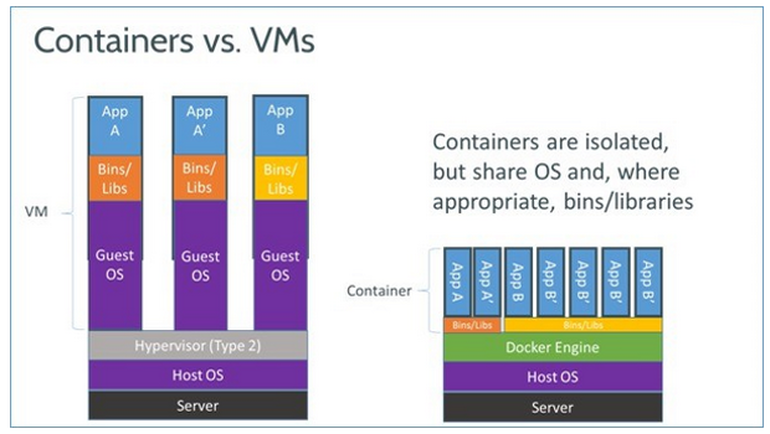
\includegraphics[width=\linewidth]{images/bab2/docker-vm-container}
	\caption{Perbandingan \textit{docker} dan virtual machine}
	\label{contohDocker}
\end{figure}
\subsection{\textit{Docker Container}}
\textit{Docker container} atau kontainer \textit{docker} bisa dikatakan sebagai sebuah wadah atau tempat, dimana kontainer \textit{docker} ini dibuat dengan menggunakan \textit{docker image}. Saat kontainer \textit{docker} dijalankan, maka akan terbentu sebuah \textit{layer} di atas \textit{docker image}.Contohnya saat menggunakan \textit{image} Ubuntu, kemudian membuat sebuah kontainer \textit{docker} dari \textit{image} Ubuntu tersebut dengan nama mitmproxy-ubuntu. Setelah itu dilakukan pemasangan sebuah perangkat lunak, misalnya \textit{mitmproxy}, maka secara otomatis kontainer \textit{docker} mitmproxy-ubuntu akan berada di atas \textit{layer image} Ubuntu, dan diatasnya lagi merupakan \textit{layer mitmproxy} berada. \textit{Docker Kontainer} atau Kontainer \textit{docker} ke depannya dapat digunakan untuk menghasilkan sebuah \textit{docker images}. \textit{Docker images} yang dihasilkan dari kontainer \textit{docker} itu sendiri nantinya dapat digunakan kembali untuk membuat kontainer \textit{docker} yang lainnya.

\subsection{\textit{Docker Images}}
\textit{Docker images} adalah sebuah \textit{blueprint} atau rancangan dasar dari sebuah perangkat lunak berbasis \textit{docker} yang bersifat \textit{read-only}. \textit{Blueprint} ini sendiri merpakan sebuah sistem operasi atau sistem operasi yang telah dipasang berbagai perangkat lunak dan pustaka pendukung. \textit{Docker iamges} berfungsi untuk membuat kontainer \textit{docker}, dimana dengan menggunakan satu \textit{docker iamge} dapat dibuat lebih dari satu kontainer \textit{docker}. \textit{Docker image} sendiri dapat menyelesaikan permasalahan yang dikenal dengan "\textit{dependency hell}", dimana sulitnya untuk melengkapi dependensi sebuah perangkat lunak. Permasalahan tersebut dapat diselesaikan karena semua kebutuhan perangkat lunak sudah berada di dalamnya.

\subsection{\textit{Docker Registry}}
\textit{Docker Registry} adalah kumpulan dari berbagai macam \textit{docker image} yang bersifat tertutup maupun terbuka yang dapat diakses di \texttt{https://hub.docker.com/} atau dapat diakses pada \textit{server} sendiri. Dengan menggunakan \textit{docker registry}, seseorang dapat menggunakan \textit{docker image} yang telah dibuat oleh orang lainnya. Hal seperti ini dapat mempermudah seseorang untuk melakukan pengembangan dan jugatransfer aplikasi.

	\chapter{DESAIN DAN PERANCANGAN}
Pada bab ini dibahas mengenai analisis dan perancangan dari sistem. 
\section{Deskripsi Umum Sistem}    
Sistem yang akan dibuat adalah sebuah sebuah sistem yang dapat membuat sebuah kontainer \textit{docker} secara otomatis untuk setiap satu \textit{client} yang telah \textit{login} ke dalam sistem. Saat \textit{client} belum \textit{login} ke dalam sistem, maka \textit{client} tersebut akan diarahkan ke halaman \textit{login} dari sistem. Saat \textit{client} mencoba untuk \textit{login} ke dalam sistem, maka sistem akan melakukan pengecekan di dalam basis data apakah \textit{username} dan \textit{password} yang di\textit{input}kan sudah benar atau salah. 

Setelah \textit{client} berhasil \textit{login} ke dalam sistem, sistem akan mengirimkan perintah untuk membuat kontainer \textit{docker} yang berisikan Mitmproxy ke \textit{docker host}. Setelah berhasil membuat kontainer \textit{docker} untuk client tersebut, maka \textit{traffic} internet dari \textit{client} tersebut akan diarahkan ke kontainer \textit{docker} berisikan Mitmproxy yang baru saja dibuat. Setelah itu client dapat mengakses internet.

\section{Kasus Penggunaan}
Terdapat empat aktor dalam sistem yang akan dibuat yaitu \textit{Client}, \textit{Server Login}, \textit{Administrator}, dan \textit{Docker Host}. \textit{Client} adalah aktor yang melakukan proses \textit{login} ke dalam sistem, \textit{server login} adalah aktor yang melakukan proses permintaan penyediaan kontainer \textit{docker}, \textit{administrator} adalah aktor yang melakukan monitoring kontainer \textit{docker} yang sedang berjalan, sedangkan \textit{docker host} adalah aktor yang akan menjadi tempat penyedia kontainer dan menerima perintah penyediaan kontainer. Diagram kasus penggunaan menggambarkan kebutuhan - kebutuhan yang harus dipenuhi sistem. Diagram kasus penggunaan digambarkan pada Gambar \ref{gambarDiagramKasusPenggunaan}.
\begin{figure}[!h] % h = pasti berada di bawah teks yang ada di atas
	\centering
	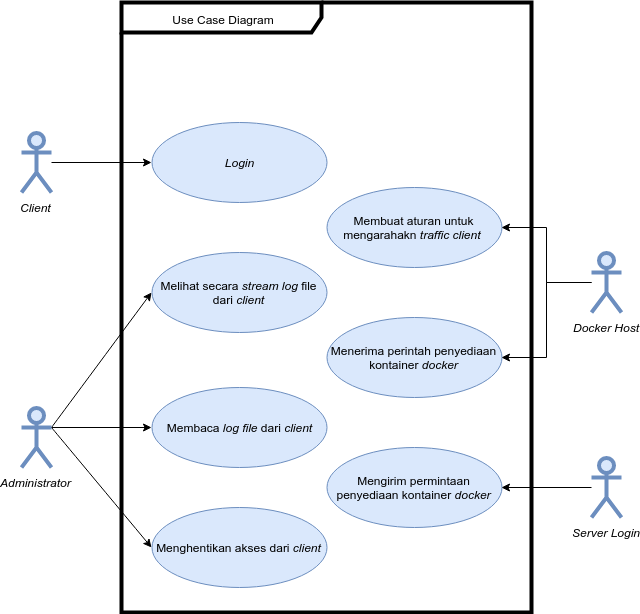
\includegraphics[width=\linewidth]{images/bab3/usecase}
	\caption{Digram Kasus Penggunaan}
	\label{gambarDiagramKasusPenggunaan}
\end{figure}
\\

Digram kasus penggunaan pada Gambar \ref{gambarDiagramKasusPenggunaan} dideskripsikan masing-masing pada Tabel \ref{tabelKodeKasusPenggunaan}.
\begin{longtable}{|p{0.25\textwidth}|p{0.24\textwidth}|p{0.35\textwidth}|} % L = Rata kiri untuk setiap kolom, | = garis batas vertikal.
	
	% Kepala tabel, berulang di setiap halaman
	\caption{Daftar Kode Kasus Penggunaan} \label{tabelKodeKasusPenggunaan} \\
	\hline
	\textbf{Kode Kasus Penggunaan} & \textbf{Nama Kasus Penggunaan} & \textbf{Keterangan} \\ \hline
	
	\endhead
	\endfoot
	\endlastfoot
	
	% Isi Tabel
	UC-0001 & \textit{Login} & \textit{Client} dapat \textit{login} ke dalam sistem. \\ \hline
	UC-0002 & Mengirim Permintaan Penyediaan Kontainer \textit{Docker} & \textit{Server login} dapat mengirimkan permintaan penyediaan kontainer \textit{docker} pada \textit{docker host}. \\ \hline
	UC-0003 & Menerima Perintah Penyediaan Kontainer \textit{Docker}  &  Proses dimana \textit{docker host} akan menerima perintah dari sistem, untuk menyediakan kontainer secara otomatis.\\ \hline
	UC-0004 & Membuat Aturan untuk Mengarahkan \textit{Traffic Client}  &  Proses dimana \textit{docker host} akan membuat aturan untuk mengarahkan \textit{traffic client} ke halaman \textit{login} dari sistem atau untuk membuat aturan untuk mengarahkan \textit{traffic client} ke kontainer \textit{docker} dari tiap-tiap \textit{client}. \\ \hline
	UC-0005 & Membaca \textit{Log File} dari \textit{Client}  &  Proses dimana \textit{administrator} dari sebuah jaringan dapat membaca \textit{log file} dari \textit{client} sampai pada \textit{client} terakhir mengakses internet.\\ \hline
	UC-0006 & Melihat Secara \textit{Stream Log File} dari \textit{Client}  &  Proses dimana \textit{administrator} dari sebuah jaringan dapat melihat \textit{log file} dari \textit{client} secara langsung atau \textit{live}.\\ \hline
\end{longtable}

\section{Arsitektur Sistem}
Pada sub-bab ini, dibahas mengenai tahap analisis arsitektur, analisis teknologi dan desain sistem yang akan dibangun.
\subsection{Desain Umum Sistem}
\indent Berdasarkan deskripsi umum sistem yang telah ditulis diatas, dapat diperoleh kebutuhan sistem ini, diantaranya :
\begin{enumerate}
	\item Pembuatan halaman \textit{login} dari sebuah sistem.
	\item Pembuatan aturan untuk mengarahkan \textit{traffic client} ke halaman \textit{login} dari sistem.
	\item Pembuatan \textit{middleware} untuk menerima permintaan dari \textit{client}.
	\item Pembuatan aturan untuk mengarahkan \textit{traffic client} ke kontainer \textit{docker} dari tiap-tiap \textit{client}.
	\item Pemasangan kontainer pada \textit{docker host}.
	\item Pembuatan halaman \textit{administrator} untuk membaca \textit{log file} dari \textit{client}.
\end{enumerate} 

\indent Untuk memenuhi kebutuhan sistem tersebut, penulis membagi sistem menjadi beberapa komponen. Komponen yang akan dibangun antara lain: 
\begin{enumerate} 
	\item Pembuatan halaman \textit{login} dari sebuah sistem.\\
	Berfungsi sebagai tampilan antarmuka dari halaman \textit{login} sebuah sistem untuk \textit{client}. Selain itu juga berfungsi untuk mengirimkan permintaan penyediaan kontainer \textit{docker} ke \textit{docker host}.
	\item Pembuatan aturan untuk mengarahkan \textit{traffic client} ke halaman \textit{login} dari sistem.\\
	Berfungsi untuk mengarahkan tiap \textit{client} yang belum \textit{login} ke dalam sistem, ke halaman \textit{login} dari sistem. Hal ini dilakukan dengan menjalankan sebuah \textit{script} dengan menggunakan Iptables pada \textit{docker host}.
	\item Pembuatan \textit{middleware} untuk menerima permintaan dari \textit{client}.\\
	Berfungsi untuk menerima permintaan pembuatan kontainer \textit{docker} dari \textit{client}. Selain itu juga berfungsi untuk membuat kontainer \textit{docker} secara otomatis.
	\item Pembuatan aturan untuk mengarahkan \textit{traffic client} ke kontainer \textit{docker} dari tiap-tiap \textit{client}.\\
	Berfungsi untuk mengarahkan \textit{traffic} dari tiap \textit{client} yang telah berhasil \textit{login}, ke kontainer \textit{docker} dari tiap-tiap \textit{client}. Hal ini dilakukan dengan menjalankan sebuah \textit{script} dengan menggunakan Iptables pada \textit{docker host}.
	\item Pemasangan kontainer pada \textit{docker host}.\\
	Berfungsi untuk memasangkan kontainer \textit{docker} pada \textit{docker host} secara otomatis. Hal ini dilakukan dengan menjalankan sebuah perintah penyediaan kontainer pada \textit{docker host}.
	\item Pembuatan halaman \textit{administrator} untuk membaca \textit{log file} dari \textit{client}.\\
	Berfungsi untuk melihat apa saja yang telak diakses oleh \textit{client}. \textit{Log} yang tersimpan terdapat \textit{log} HTTP maupun \textit{log} HTTPS.  Hal ini dilakukan dengan menjalankan sebuah perintah untuk melihat \textit{log file} dari suatu \textit{client}.
	
\end{enumerate}

\begin{figure}[H]
	\centering
	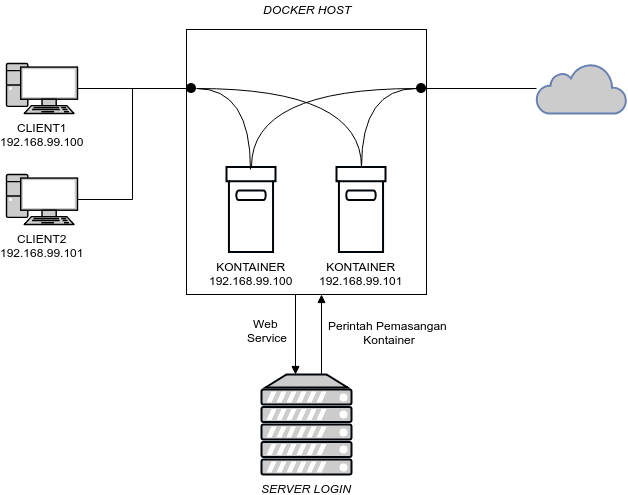
\includegraphics[width=\linewidth]{images/bab3/DIAGRAM1}
	\caption{Arsitektur Komponen Sistem}
	\label{Arsitektur Komponen Sistem}
\end{figure}

\indent Pada pada Gambar \ref{Arsitektur Komponen Sistem} ditunjukkan arsitektur sistem secara umum dengan detail-detail dari kompenen yang terdapat didalamnya. Setiap komponen tersebut akan diimplementasikan dengan teknologi pendukung yang dibutuhkan.

Nantinya tiap \textit{client}  akan mempunyai satu kontainer \textit{docker} dan satu \textit{port} secara pribadi. \textit{Traffic} dari \textit{client} tersebut akan diarahkan menuju ke kontainer \textit{docker}nya dari tiap-tiap \textit{client}, setelah itu \textit{client} baru dapat mengakses itnernet.

\subsection{Pembuatan Halaman \textit{Login} dari Sebuah Sistem.}
Pembuatan halaman \textit{login} dari sebuah sistem adalah komponen yang bertugas untuk menyediakan tampilan antarmuka dari halaman \textit{login} untuk \textit{client}. Awalnya semua \textit{traffic} diarahkan menuju ke halaman \textit{login} dari sebuah sistem, karena diasumsikan bahwa semua \textit{client} diamsumsikan belum \textit{login} ke dalam sistem. Supaya \textit{client} dapat mengakses internet, maka \textit{client} harus \textit{login} ke dalam sistem terlebih dahulu dengan memasukkan \textit{username} dan \textit{password} dari \textit{client} tersebut.

Dikarenakan ada beberapa kebutuhan yang harus dipenuhi, komponen pada pembuatan halaman \textit{login} dari sebuah sistem dibagi lagi menjadi dua sub komponen, yaitu:
\begin{enumerate}
	\item Basis Data \\
	Basis data pada komponen pembuatan halaman \textit{login} dari sebuah sistem berfungsi sebagai tempat penyimpanan data \textit{username} dan \textit{password} yang digunakan untuk \textit{login} ke dalam sistem. Basis data juga berfungsi sebagai tempat penyimpanan data kontainer \textit{docker} yang sudah dibuat.
	\item \textit{Web Service} \\
	\textit{Web service} berfungsi sebagai antarmuka untuk \textit{client} ketika \textit{client} akan \textit{login} ke dalam sistem. Selain itu \textit{web service} juga berfungsi untuk mengirimkan permintaan penyediaan kontainer \textit{docker} ke \textit{docker host} ketika terdapat \textit{client} yang telah berhasil \textit{login} ke dalam sistem.
\end{enumerate}

Pada tugas akhir ini, bahasa Python dipilih sebagai bahasa pemrograman dan Flask dipilih sebagai kerangka kerja untuk bahasa pemrograman Python yang digunakan untuk mengimplementasikannya. Lalu, pada bagian penyimpanan data atau basis data, MySQL dipilih sebagai RDBMS untuk tugas akhir ini.

\subsubsection{Desain Basis Data}
Komponen basis data berfungsi sebagai tempat penyimpanan data \textit{username} dan \textit{password} yang digunakan untuk \textit{login} ke dalam sistem. Dalam basis data ini terdapat satu entitas dan empat atribut, ditunjukkan pada Tabel \ref{tabelnrpmahasiswa}
\begin{longtable}{|p{0.03\textwidth}|p{0.20\textwidth}|p{0.20\textwidth}|p{0.41\textwidth}|}
	\caption{Atribut basis data nrp-mahasiswa} \label{tabelnrpmahasiswa} \\
	\hline
	\textbf{No} & \textbf{Kolom} & \textbf{Tipe} & \textbf{Keterangan} \\ \hline
	\endhead
	\endfoot
	\endlastfoot
	1 & id & int(11) & Sebagai primary key pada tabel, nilai awal adalah \texttt{AUTO\_INCREMENT}. \\ \hline
	2 & username & varchar(50) & Menunjukkan NRP dari mahasiswa yang telah terdaftar. \\ \hline
	3 & password & varchar(50) & Menunjukkan password dari NRP mahasiswa yang telah terdaftar. \\ \hline
	4 & isLogin & int(11) & Status apakah nrp tersebut sedang digunakan (1), atau sedang tidak digunakan (0). \\ \hline
\end{longtable}
\subsubsection{Desain \textit{Web Service}}
Komponen \textit{web service} berfungsi untuk menyediakan antar muka halaman \textit{login} untuk \textit{client} dan untuk mengirimkan permintaan pembuatan kontainer \textit{docker} secara otomatis pada \textit{docker host} setelah terdapat \textit{client} yang berhasil \textit{login} ke dalam sistem. Halaman \textit{login} akan menggunakan Material UI untuk mendapatkan tampilan yang sederhana dan nyaman untuk digunakan. Desain \textit{web service} untuk halaman \textit{login} dari sistem dapat dilihat pada Gambar \ref{mockuplogin}.

\begin{figure}[H]
	\centering
	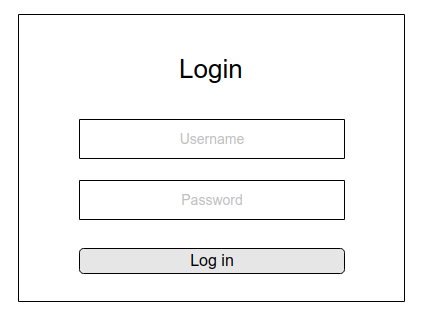
\includegraphics[width=\linewidth]{images/bab3/MockupLogin}
	\caption{Desain Halaman \textit{Login}}
	\label{mockuplogin}
\end{figure}

Lalu untuk desain \textit{backend} dari \textit{web serive} untuk halaman \textit{login} akan menggunakan bahasa pemrograman Python degan kerangka kerja Flask yang akan dijalankan dengan Gunicorn. Kemudian Gunicorn akan dijalankan dengan Supervisor sebagai \textit{service}. Lalu akan digunakan \textit{nginx} sebagai \textit{web server} dari halaman \textit{login} dari sebuah sistem. Desain \textit{backend} dari \textit{web service} untuk halaman \textit{login} dapat dilihat pada Gambar \ref{desainbackendhalamanlogin}.

\begin{figure}[H]
	\centering
	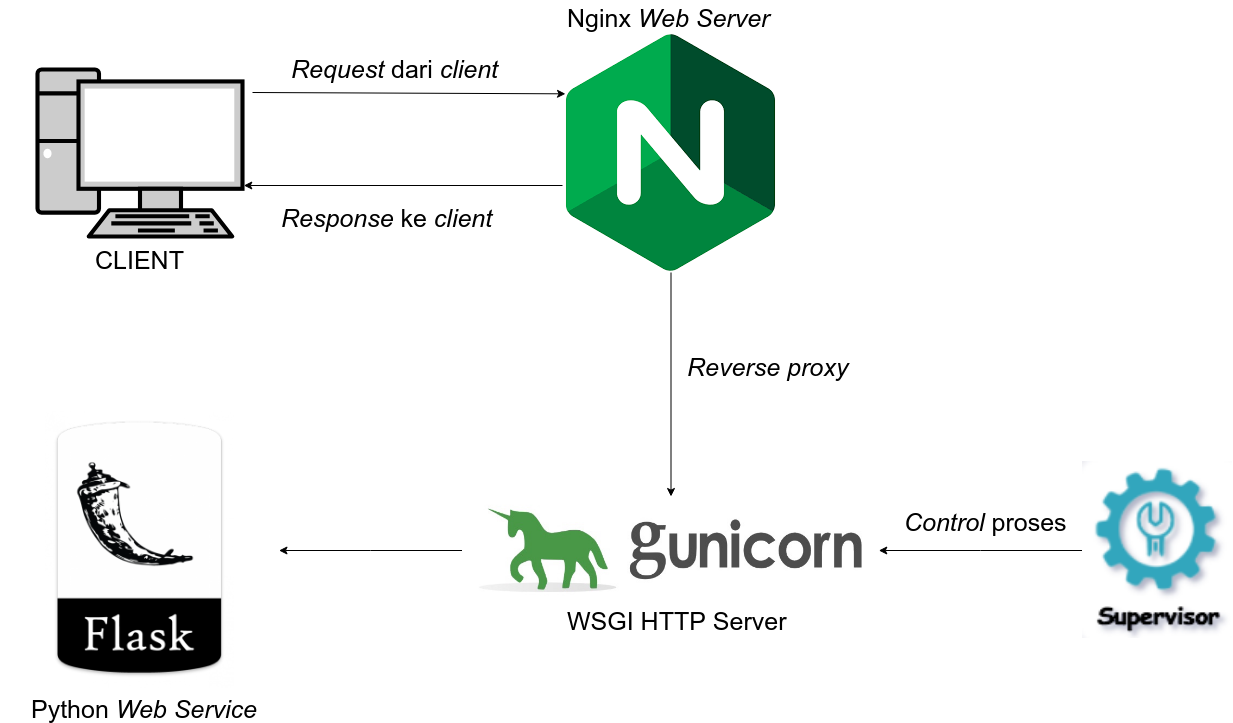
\includegraphics[width=\linewidth]{images/bab3/DesainBackend}
	\caption{Desain \textit{Backend} dari Halaman \textit{Login}}
	\label{desainbackendhalamanlogin}
\end{figure}

\subsection{Perancangan Pembuatan Aturan untuk Mengarahkan \textit{Traffic Client} ke Halaman \textit{Login} dari Sistem}
Pembuatan aturan untuk mengarahkan \textit{traffic client} ke halaman \textit{login} dari sistem adalah komponen yang bertugas untuk membelokkan \textit{traffic} dari \textit{client} yang akan menuju ke internet. Awalnya semua \textit{traffic} dari satu \textit{subnet client} tersebut akan diarahkan ke halaman \textit{login} dari sistem dengan membuat sebuah aturan menggunakan Iptables, karena asumsinya adalah belum ada \textit{client} yang berhasil \textit{login} ke dalam sistem. Desain perancangan pembuatan aturan untuk mengarahkan \textit{traffic client} ke halaman \textit{login} dapat dilihat pada Gambar \ref{dessainmengarahkankehalamanlogin} .
\begin{figure}[H]
	\centering
	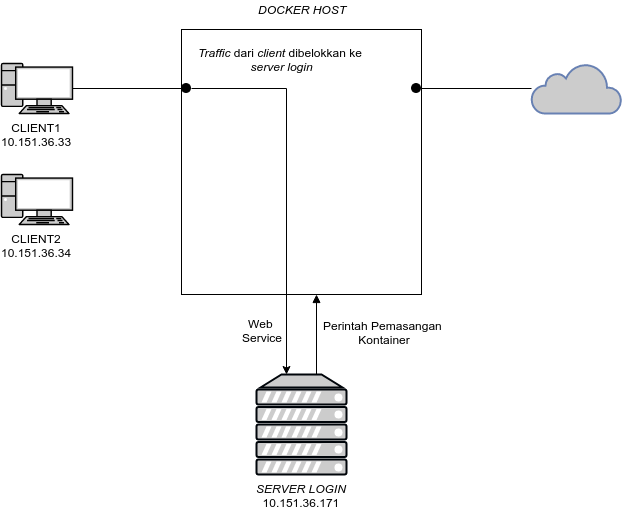
\includegraphics[width=\linewidth]{images/bab3/DIAGRAM2}
	\caption{Desain Mengarahkan \textit{Traffic Client} ke Halaman \textit{Login}}
	\label{dessainmengarahkankehalamanlogin}
\end{figure}

\subsection{Pembuatan \textit{Middleware} untuk Menerima Permintaan dari \textit{Client}}
Pembuatan \textit{middleware} untuk menerima permintaan dari \textit{client} adalah komponen yang bertugas untuk menerima permintaan dari \textit{client} yang telah berhasil \textit{login} ke dalam sistem. Permintaan yang dikirimkan oleh \textit{client} adalah permintaan untuk membuat kontainer \textit{docker} secara otomatis. Nantinya setiap satu \textit{client} yang berhasil \textit{login} ke dalam sistem akan dibuatkan satu kontainer \textit{docker}.

Dikarenakan ada beberapa kebutuhan yang harus dipenuhi, komponen pada pembuatan \textit{middleware} untuk menerima permintaan dari \textit{client} dibagi lagi menjadi dua buah komponen, yaitu:

\begin{enumerate}
	\item Basis Data \\
	Basis data  berfungsi sebagai tempat penyimpanan data kontainer \textit{docker} yang sudah dibuat.
	\item \textit{Web Service} \\
	\textit{Web service} berfungsi sebagai penerima permintaan dari \textit{client}, yang nantinya akan membuat sebuah kontainer \textit{docker} secara otomatis pada \textit{docker host}.
\end{enumerate}

Sama seperti komponen pembuatan halaman \textit{login} dari sebuah sistem, pada tugas akhir ini, bahasa Python dipilih sebagai bahasa pemrograman yang digunakan untuk mengimplementasikannya. Lalu, pada bagian penyimpanan data atau basis data, MySQL dipilih sebagai RDBMS untuk tugas akhir ini. 

\subsubsection{Desain Basis Data}
Komponen basis data berfungsi sebagai tempat penyimpanan data kontainer \textit{docker} yang sudah dibuat. Dalam basis data ini terdapat satu entitas dan empat atribut, ditunjukkan pada Tabel \ref{tabelkontainer}.

\begin{longtable}{|p{0.03\textwidth}|p{0.20\textwidth}|p{0.20\textwidth}|p{0.41\textwidth}|}
	\caption{Atribut basis data kontainer} \label{tabelkontainer} \\
	\hline
	\textbf{No} & \textbf{Kolom} & \textbf{Tipe} & \textbf{Keterangan} \\ \hline
	\endhead
	\endfoot
	\endlastfoot
	1 & id & int(11) & Sebagai primary key pada tabel, nilai awal adalah \texttt{AUTO\_INCREMENT}. \\ \hline
	2 & username & varchar(50) & Menunjukkan NRP dari mahasiswa yang telah berhasil dibuatkan satu kontainer \textit{docker}. \\ \hline
	3 & ip & varchar(50) & Menunjukkan IP dari \textit{client} yang telah berhasil dibuatkan satu kontainer \textit{docker}. \\ \hline
	4 & port & varchar(50) & Menunjukkan \textit{port} dari \textit{client} yang telah berhasil dibuatkan satu kontainer \textit{docker}. \\ \hline
	5 & createdAt & datetime & Menunjukkan waktu pertama kali kontainer \textit{docker} tersebut dibuat. \\ \hline
	
\end{longtable}


\subsubsection{Desain \textit{Web Service}}
Komponen \textit{web service} berfungsi untuk menerima permintaan dari \textit{client} untuk membuat satu kontainer \textit{docker} pada \textit{docker host}. Kontainer \textit{docker} yang akan dibuat pada \textit{docker host} akan dibuat secara otomatis oleh sistem, dan kontainer \textit{docker} yang dibuat akan memiliki nama sesuai dengan IP dari \textit{client} yang telah berhasil \textit{login} ke dalam sistem. Setelah menerima permintaan dari \textit{client}, maka sistem akan mengirimkan perintah untuk membuat kontainer \textit{docker} khusus untuk satu \textit{client}. 

\subsection{Perancangan Pemasangan Kontainer pada \textit{Docker Host}}
Pemasangan kontainer adalah kompenen yang berfungsi untuk memasang kontainer \textit{docker} yang berisi Mitmproxy pada \textit{docker host} setelah ada permintaan dari \textit{client} yang telah berhasil \textit{login} ke dalam sistem. Proses ini dilakukan secara otomatis, dan nama dari kontainer \textit{docker} tersebut akan sesuai dengan IP dari \textit{client} yang telah berhasil \textit{login} ke dalam sistem.

Saat kontainer \textit{docker} telah berhasil dibuat, maka kontainer \textit{docker} tersebut akan mempunyai satu \textit{port} khusus yang sama dengan \textit{client} yang baru saja \textit{login}. \textit{Port} khusus nantinya akan digunakan untuk mengarahkan \textit{traffic} dari \textit{client} yang akan mengakses internet.

\textit{Image} Mitmproxy dipilih sebagai \textit{image} pada kontainer \textit{docker} karena Mitmproxy merupakan sebuah perangkat lunak yang interaktif dimana Mitmproxy memungkinkan dapat memotong dan memodifikasi HTTP \textit{requests} atau \textit{response} dengan sangat cepat. Mitmproxy sendiri juga dapat berjalan dengan \textit{transparent mode} sehingga \textit{client} tidak mengetahui jika \textit{traffic} dari \textit{client} tersebut ternyata melalui Mitmproxy. Gambar alur kerja dari Mitmproxy dengan \textit{transparent mode} untuk HTTP dapat dilihat pada Gambar \ref{mitmproxyhttp}.

\begin{figure}[H]
	\centering
	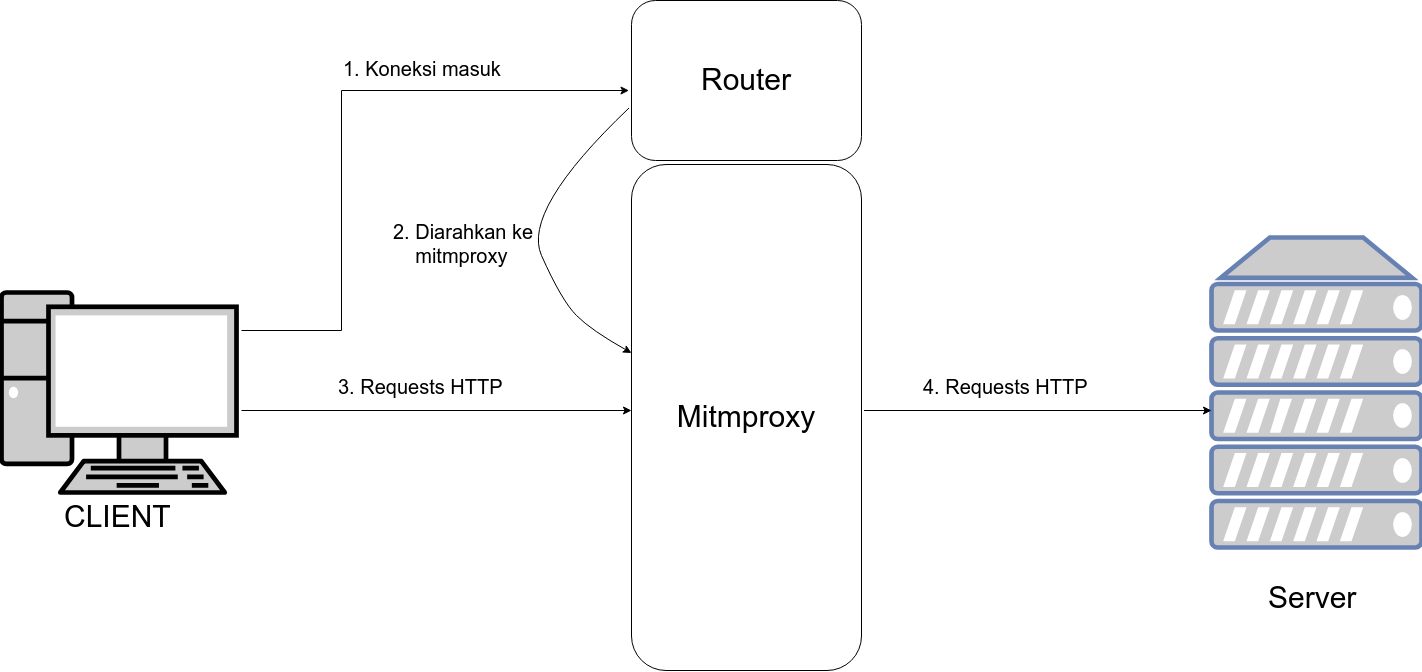
\includegraphics[width=\linewidth]{images/bab3/mitmproxyhttp}
	\caption{Alur kerja dari \textit{mitmproxy transparent} HTTP}
	\label{mitmproxyhttp}
\end{figure}

Sedangkan gambar alur kerja dari Mitmproxy dengan \textit{transparent mode} untuk HTTPS dapat dilihat pada Gambar \ref{mitmproxyhttps}.

\begin{figure}[H]
	\centering
	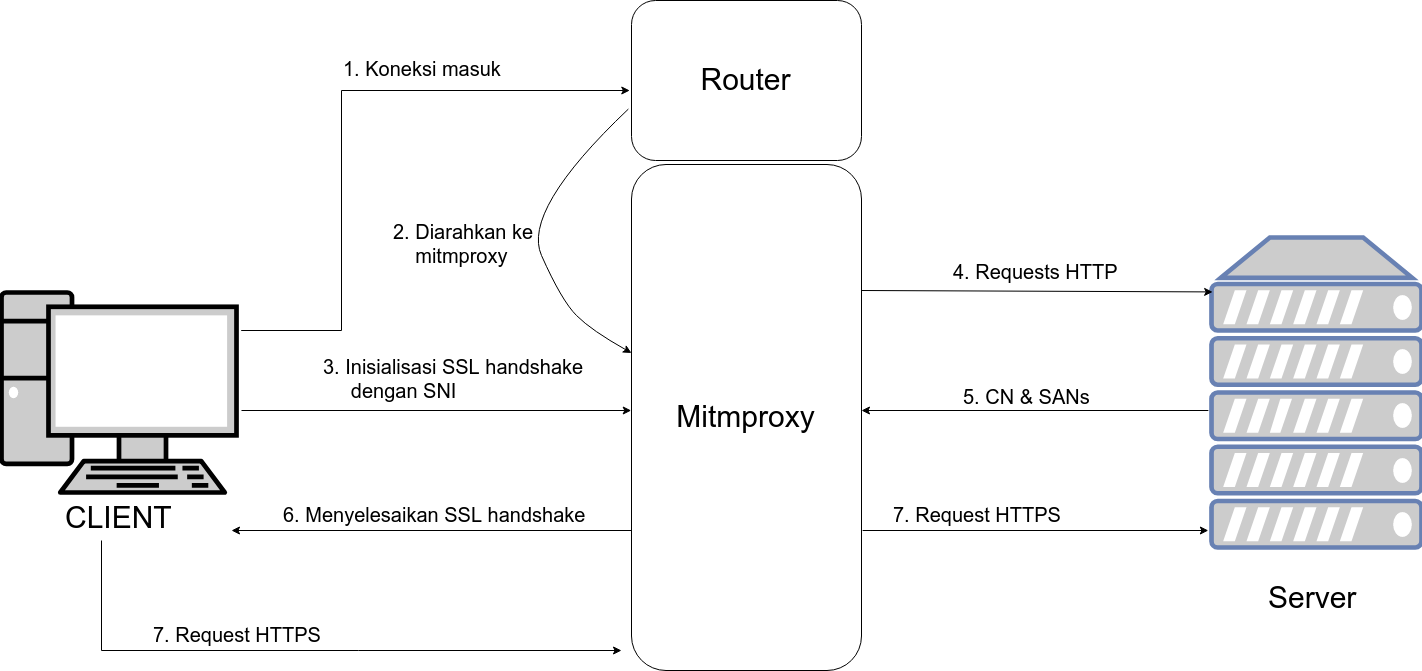
\includegraphics[width=\linewidth]{images/bab3/mitmproxyhttps}
	\caption{Alur kerja dari \textit{mitmproxy transparent} HTTPS}
	\label{mitmproxyhttps}
\end{figure}

\subsection{Pembuatan Aturan untuk Mengarahkan \textit{Traffic Client} ke Kontainer \textit{Docker} dari Tiap-Tiap \textit{Client}}
Pembuatan aturan untuk mengarahkan \textit{traffic client} ke kontainer \textit{docker} dari tiap-tiap \textit{client} adalah komponen yang bertugas untuk mengarahkan satu client ke satu kontainer \textit{docker} yang sesuai. Setelah \textit{client} berhasil \textit{login} ke dalam sistem, maka aturan ini akan dibuat menggunakan Iptables. Lalu \textit{client} juga akan diberikan sebuah aturan dengan menggunakan Iptables yang memperbolehkan \textit{client} tersebut mengakses internet. Desain dari pembuatan aturan untuk mengarahkan \textit{traffic client} ke kontainer \textit{docker} dari tiap-tiap \textit{client} dapat dilihat pada Gambar \ref{mengarahkankontainerdocker}.

\begin{figure}[H]
	\centering
	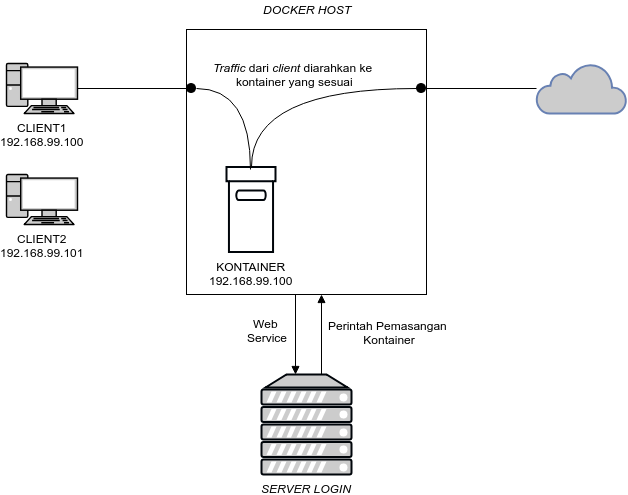
\includegraphics[width=\linewidth]{images/bab3/DIAGRAM3}
	\caption{Desain pembuatan aturan untuk mengarahkan \textit{traffic client} ke kontainer \textit{docker}}
	\label{mengarahkankontainerdocker}
\end{figure}

\subsection{Pembuatan Halaman \textit{Administrator} untuk Membaca \textit{Log File} dari \textit{Client}}
Pembuatan halaman \textit{administrator} untuk membaca \textit{log file} dari \textit{cient} adalah komponen yang bertugas untuk mengunduh \textit{log file} dari \textit{client} dan juga untuk membaca \textit{log file} dari \textit{client} secara langsung atau \textit{live} maupun hanya pada saat \textit{client} terakhir mengakses internet.

Halaman \textit{administrator} akan menggunakan Boostsrap 4 untuk mendapatkan tampilan yang sederhana dan nyaman untuk digunakan. Desain dari halaman \textit{administrator} dapat dilihat pada Gambar \ref{desaindashboard} dan Gambar \ref{desainstream} .

\begin{figure}[H]
	\centering
	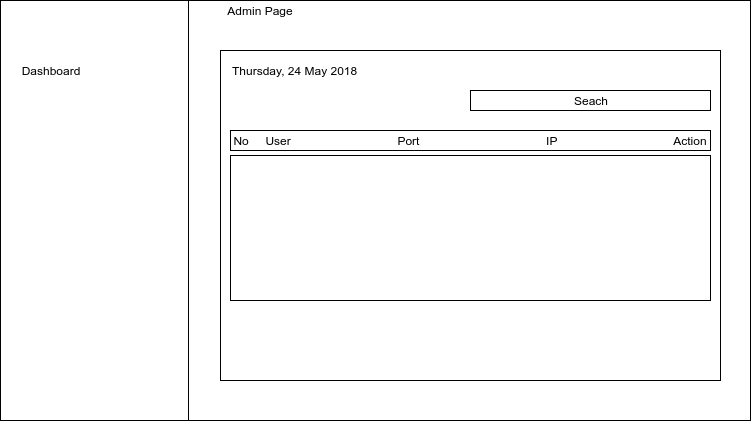
\includegraphics[width=\linewidth]{images/bab3/desaindashboard}
	\caption{Desain halaman dashboard \textit{administrator} \textit{traffic client} ke kontainer \textit{docker}}
	\label{desaindashboard}
\end{figure}

\begin{figure}[H]
	\centering
	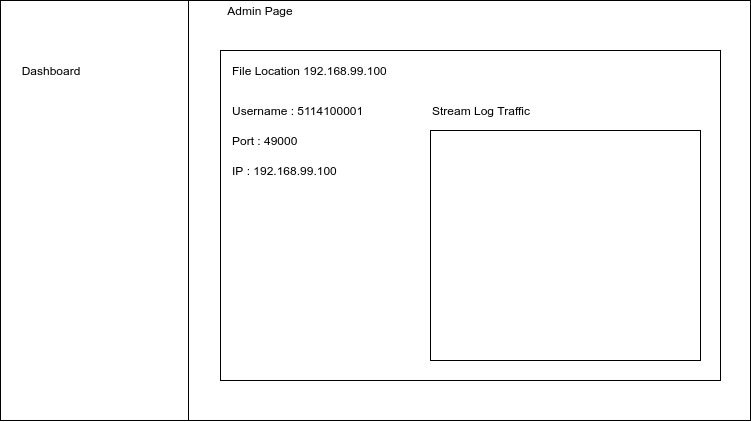
\includegraphics[width=\linewidth]{images/bab3/desainstream}
	\caption{Desain pembuatan aturan untuk mengarahkan \textit{traffic client} ke kontainer \textit{docker}}
	\label{desainstream}
\end{figure}



	\chapter{IMPLEMENTASI}
Setelah melewati proses perancangan mengenai sistem yang akan dibuat, maka akan dilakukan implementasi dari sistem tersebut. Bab ini akan membahas mengenai implementasi dari sistem yang meliputi proses pembuatan setiap komponen sehingga sistem dapat berjalan dengan baik. Masing-masing proses pembuat komponen akan dilengkapi dengan \textit{pseudocode} atau konfigurasi dari sistem.  
\section{Lingkungan Implementasi}
Dalam mengimplementasikan sistem, digunakan beberapa perangkat pendukung sebagai berikut.
\subsection{Perangkat Keras}
Perangkat keras yang digunakan dalam pengembangan sistem adalah sebagai berikut:
\begin{enumerate}
	\item Komputer dengan \textit{processor} Intel(R) Core(TM) i5-2120 CPU @ 3.30GHz dan RAM 8GB
	\item Dua Komputer dengan \textit{processor} Intel(R) Core(TM)2 Duo CPU E7200 @ 2.53GHz dan RAM 1GB
\end{enumerate}
\subsection{Perangkat Lunak}
Perangkat lunak yang digunakan dalam pengembangan sistem adalah sebagai berikut:
\begin{enumerate}
	\item Sistem Operasi Linux Mint 18.03 64 Bit sebagai \textit{docker host}.
	\item Sistem Operasi Ubuntu 14.04 LTS 64 Bit sebagai \textit{client}.
	\item Sistem Operasi Ubuntu Server 16.04 LTS 64 Bit sebagai \textit{server login}.
	\item \textit{Python} versi 3.5.2 untuk pengembangan web service. 
	\item \textit{Flask} versi 1.0.2 sebagai kerangka kerja \textit{Python}.
	\item \textit{Gunicorn} versi 19.8.1
	\item \textit{Supervisor} versi 3.2.0
	\item \textit{Nginx} versi 1.10.3
	\item \textit{Mitmproxy} versi 3.0.4 untuk mencatat semua \textit{traffic} dari \textit{client}.
	\item MySQL versi 5.7.18 untuk Sistem Manajemen Basis Data.
	\item \textit{Docker} versi 1.13.1 sebagai kontainer yang akan di pasangkan pada \textit{server}.
	\item \textit{Iptables} versi 1.6.0 untuk membuat aturan terhadap \textit{client}.
	\item \textit{Laravel} versi 5.4 sebagai kerangka kerja untuk halaman \textit{administrator}. 
	\item \textit{VIM} versi 7.4.1 sebagai \textit{text editor}.
\end{enumerate}

\section{Implementasi Pembuatan Halaman \textit{Login} dari Sebuah Sistem}
Halaman \textit{login} dibangun pada sebuah \textit{server} dengan IP \texttt{10.151.36.173} dengan menggunakan sistem operasi Ubuntu Server 16.04 LTS 64 Bit. Pada implementasi pembuatan halaman \textit{login} dari sebuah sistem menggunakan perangkat lunak antara lain:
\begin{enumerate}
	\item \textit{Python} versi 3.5.2.
	\item \textit{Flask} versi 1.0.2.
	\item \textit{Gunicorn} versi 19.8.1.
	\item \textit{Supervisor} versi 3.2.0.
	\item \textit{Nginx} versi 1.10.3.
\end{enumerate}

Lalu sistem operasi yang digunakan adalah sistem operasi Ubuntu Server 16.04 LTS 64 Bit, yang akan dipasang pada \textit{virtual machine} di \textit{Proxmox}. \textit{Python} akan berfungsi sebagai komponen dasar pembangunan sistem yang akan dibangun dengan menggunakan kerangka kerja \textit{Flask} dan dijalankan dengan \textit{Gunicorn} pada \textit{server} dengan IP \texttt{10.151.36.173} dengan \textit{port} 4000. Lalu \textit{Supervisor} akan berfungsi sebagai sebuah \textit{service} yang akan selalu menajalankan \textit{Gunicorn}. Sedangkan \textit{Nginx} akan berfungsi sebagai \textit{web server} untuk perangkat lunak halaman \textit{login} yang dijalankan oleh \textit{Gunicorn} pada \textit{server} dengan IP \texttt{10.151.36.173} dengan \textit{port} 4000 supaya bisa diakses oleh \textit{client}. Implementasi pembuatan halaman \textit{login} dari sebuah sistem akan terbagi menjadi implementasi \textit{web service} dan implementasi basis data.

\subsection{Implementasi \textit{Web Service} pada Halaman \textit{Login}}
Diperlukan beberapa tahap, antara lain pemasangan perangkat lunak dan tahap konfigurasi. Tahap pemasangan perangkat lunak dan tahap konfigurasi pada \textit{server} untuk halaman \textit{login} dijelaskan pada Lampiran A. 

Perlu diperhatikan ketika menambahkan atau mengubah konfigurasi \textit{Supervisor} pada \texttt{/etc/supervisor/conf.d/} di \textit{server} untuk halaman \textit{login}, perlu dilakukan \textit{reload Supervisor} dengan menjalankan \textit{command} pada terminal seperti pada Kode Sumber \ref{reloadsupervisor}.
\begin{lstlisting}[frame=single,tabsize=2,breaklines,caption=Command untuk Reload Supervisor,language=Python,label=reloadsupervisor,captionpos=b]
sudo supervisorctl reread
sudo supervisorctl reload
sudo supervisorctl status
\end{lstlisting}

Perlu diperhatikan pula ketika menambahkan atau mengubah konfigurasi \textit{Nginx} pada \texttt{/etc/nginx/sites-available/} di \textit{server} untuk halaman \textit{login}, perlu dilakukan aktifasi konfigurasi \textit{Nginx} dengan menjalankan \textit{command} pada terminal seperti pada Kode Sumber \ref{aktifasikonfigurasinginx}.
\begin{lstlisting}[frame=single,tabsize=2,breaklines,caption=Command untuk mengaktifkan konfigurasi Nginx,language=Python,label=aktifasikonfigurasinginx,captionpos=b]
sudo ln -s /etc/nginx/sites-available/app 
	/etc/nginx/sites-enabled/app
\end{lstlisting}

Setelah itu, jalankan Kode Sumber \ref{restartnginx} supaya konfigurasi yang baru saja diaktifkan dapat digunakan.\\
\begin{lstlisting}[frame=single,tabsize=2,breaklines,captionpos=b,caption=Command untuk merestart Nginx,language=Python,label=restartnginx]
sudo service nginx restart
\end{lstlisting}

\subsubsection{Implementasi Tampilan Antarmuka Halaman \textit{Login}}
Halaman \textit{login} merupakan halaman utama yang menampilkan sebuah \textit{form input} untuk \textit{client}. Pada halaman ini terdapat dua \textit{form input}, yaitu \textit{form input} untuk \texttt{Username} atau NRP dari \textit{client} dan juga \textit{form input} untuk \texttt{Password} dari \textit{client}. Implementasi antarmuka halaman \textit{login} dapat dilihat pada Gambar \ref{implementasihalamanlogin}.

\begin{figure}[H]
	\centering
	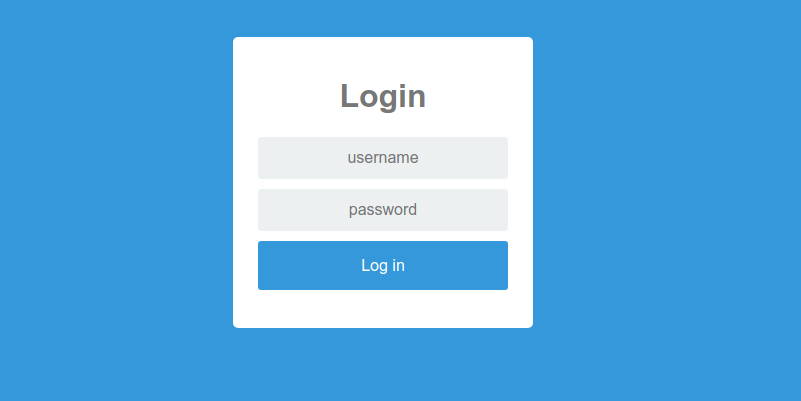
\includegraphics[width=\linewidth]{images/bab4/halamanlogin}
	\caption{Halaman \textit{Login}}
	\label{implementasihalamanlogin}
\end{figure}

\subsubsection{Rute \textit{Web Service} pada Halaman \textit{Login}}
Pada halaman \textit{login} diperlukan adanya rute-rute yang bisa diakses untuk melayani \textit{client}, supaya \textit{client} dapat membuka tampilan antar muka dari halaman \textit{login} dan juga supaya \textit{client} dapat mengirimkan permintaan untuk membuat kontainer \textit{docker} pada \textit{docker host}. Daftar rute yang disediakan oleh halaman \textit{loign} tertera pada Tabel \ref{tabelRuteWebServiceHalamnLogin}.\\
\begin{longtable}{|p{0.15\textwidth}|p{0.25\textwidth}|p{0.4\textwidth}|p{0.3\textwidth}|} % L = Rata kiri untuk setiap kolom, | = garis batas vertikal.
	
	% Kepala tabel, berulang di setiap halaman
	\caption{Daftar Rute \textit{Web Service}} \label{tabelRuteWebServiceHalamnLogin} \\
	\hline
	\textbf{HTTP Method} & \textbf{Rute} & \textbf{Deskripsi} \\ \hline
	
	\endfirsthead
	\caption[]{Daftar Rute \textit{Web Service}}  \\
	\hline
	\textbf{HTTP Method} & \textbf{Rute} & \textbf{Deskripsi}  \\ \hline
	
	\endhead
	\endfoot
	\endlastfoot
	
	% Isi Tabel
	GET & / & Berfungsi untuk mengarahkan \textit{redirect} ke rute \textit{login} dengan \textit{method} GET.\\ \hline
	GET & /login & Berfungsi untuk menampilkan tampilan grafis antar muka halaman \textit{login} ketika \textit{client} belum \textit{login} ke dalam sistem dan untuk menampilkan tampilan grafis antar muka halaman sukses \textit{login} ketika \textit{client} telah berasil \textit{login} ke dalam sistem.\\ \hline
	POST & /login & Berfungsi untuk menyimpan data hasil \textit{input} dari \textit{client} dan mengirimkan perintah untuk membuat kontainer \textit{docker} yang berisikan \textit{mitmproxy} secara otomatis pada \textit{docker host}.\\ \hline
\end{longtable}

\subsubsection{\textit{Pseduocode Web Service} pada Halaman \textit{Login}}
Ketika \textit{client} belum \textit{login} ke dalam sistem, maka akan diarahkan ke tampilan grafis antar muka dari halaman \textit{login}. Lalu setelah \textit{client} berhasil \textit{login} ke dalam sistem, maka akan diarahkan ke tampilan grafis antar muka halaman sukses \textit{login}. Pada Kode Sumber \ref{pseudocodehalamanlogin} diperlihatkan bagaimana implementasinya dalam bentuk \textit{pseduocode}.

\begin{minipage}{\linewidth}  
	\begin{lstlisting}[numbers=left, frame=single,tabsize=2,breaklines,caption={Pseudocode Web Service},label=pseudocodehalamanlogin,language=json]
	Check whether the client is already login or not yet
	
	if session.get login
		open welcome page
	else
		open login page
		if login success
			session.get login = True	  
	
	return  	
	\end{lstlisting}
\end{minipage}


\subsection{Implementasi Basis Data pada Halaman \textit{Login}}
Berdasarkan hasil desain dan perancangan basis data pada bab 3 terdapat satu entitas yang diimplementasikan menjadi suatu tabel pada basis data MySQL, yaitu entitas \texttt{nrp-mahasiswa}. Detail implementasi \textit{query} untuk membuat basis data dengan entitas \texttt{nrp-mahasiswa} seperti pada Kode Sumber \ref{entitasnrpmahasiswa}.\\
\begin{lstlisting}[frame=single,tabsize=2,breaklines,captionpos=b,language=python, caption=\textit{Query} untuk membuat tabel testing,label=entitasnrpmahasiswa]
CREATE TABLE nrp-mahasiswa (
	id int(11) PRIMARY KEY AUTO_INCREMENT,
	nrp VARCHAR(50)
	password VARCHAR(50)
	isLogin int(11)
);
\end{lstlisting}


\section{Implementasi Pembuatan Aturan untuk Mengarahkan \textit{Traffic Client} ke Halaman \textit{Login} dari Sistem}
Pada implementasi pembuatan aturan untuk mengarahkan \textit{traffic client} ke halaman \textit{login} dari sistem diasumsikan bahwa belum ada \textit{client} yang telah \textit{login} ke dalam sistem. Karena diasumsikan bahwa belum ada \textit{client} yang telah berhasil \textit{login} ke dalam sistem, maka semua \textit{client} tidak diperbolehkan untuk mengakses internet. Kemudian untuk mengarahkan \textit{traffic} dari \textit{client} dibuatkan beberapa \textit{rules} dengan menggunakan \textit{iptables} pada \textit{Docker Host} dengan IP \texttt{10.151.36.134}. seperti Kode Sumber \ref{iptablesbeforelogin}.
\begin{lstlisting}[frame=single,tabsize=2,breaklines,captionpos=b,caption=Command untuk mengarahkan \textit{client} ke halaman \textit{login},language=Python,label=iptablesbeforelogin]
iptables -I FORWARD 1 -s 192.168.99.0/24 -j REJECT
iptables -I FORWARD 1 -s 192.168.99.0/24 -p tcp d 10.151.36.173 --dport 4000 -j ACCEPT
iptables -t nat -I PREROUTING 1 -p tcp -s 192.168.99.0/24 --dport 80 -j DNAT --to 10.151.36.173:4000
\end{lstlisting}

\indent \textit{Rules} pertama berfungsi untuk melarang semua \textit{client} untuk melewati \textit{router}. \textit{Rules} kedua berfungsi untuk mengizinkan semua \textit{client} membuka halaman \textit{login}. Sedangkan \textit{rules} ketiga berfungsi untuk mengarahkan semua \textit{traffic client} ke halaman \textit{login}.

\section{Implementasi Pembuatan \textit{Middleware}}
\textit{Middleware} dibangun pada \textit{Docker Host} dengan IP \texttt{10.151.36.134} dengan menggunakan sistem operasi Linux Mint 18.03 64 Bit. \textit{Middleware} merupakan komponen yang akan menerima permintaan dari \textit{client}, mengirimkan perintah untuk membuat kontainer \textit{docker} secara otomatis pada \textit{docker host}, dan menentukan rute \textit{traffic} dari \textit{client} menuju ke internet sesuai kontainer \textit{docker} masing-masing user. Implementasi \textit{middleware} akan terbagi menjadi implementasi basis data dan implementasi \textit{web service}.

Pada implementasi pembuatan \textit{middleware} menggunakan perangkat unak antara lain:
\begin{enumerate}
	\item \textit{Python} versi 3.5.2.
	\item \textit{Flask} versi 1.0.2.
	\item \textit{Docker} versi 1.13.1.
\end{enumerate}

\textit{Python} akan berfungsi sebagai komponen dasar pembangunan sistem, salah satunya adalah sebagai komponen dasar pembuatan \textit{middleware}, sedangkan \textit{Flask} akan berfungsi sebagai kerangka kerja untuk pembuatan \textit{middleware}. Implementasi pembuatan \textit{middleware} akan terbagi menjadi implementasi \textit{web service} dan implementasi basis data dan.

\subsection{Implementasi \textit{Web Service} pada \textit{Middleware}}
Diperlukan beberapa tahap, antara lain pemasangan perangkat lunak dan tahap konfigurasi. Tahap pemasangan perangkat lunak dan tahap konfigurasi pada \textit{middleware} di \textit{Docker Host} dijelaskan pada Lampiran B.

Perlu diperhatikan supaya \textit{docker} dapat dijalankan ketika \textit{docker host} menyala, jalankan Kode Sumber \ref{systemctldocker}.
\begin{lstlisting}[frame=single,tabsize=2,breaklines,captionpos=b,caption=Command untuk installasi Flask,language=Python,label=systemctldocker]
sudo systemctl enable docker
\end{lstlisting}

\subsubsection{Rute \textit{Web Service} pada \textit{Middleware}}
\textit{Middleware} tidak memiliki antar muka grafis. Namun tetap diperlukan adanya rute-rute yang bisa diakses untuk melayani permintaan penyediaan kontainer \textit{docker} dari \textit{client}. Daftar rute yang disediakan oleh \textit{middleware} tertera pada Tabel \ref{tabelRuteWebServiceDockerHost}.\\
\begin{longtable}{|p{0.15\textwidth}|p{0.25\textwidth}|p{0.4\textwidth}|p{0.3\textwidth}|} % L = Rata kiri untuk setiap kolom, | = garis batas vertikal.
	
	% Kepala tabel, berulang di setiap halaman
	\caption{Daftar Rute \textit{Web Service}} \label{tabelRuteWebServiceDockerHost} \\
	\hline
	\textbf{HTTP Method} & \textbf{Rute} & \textbf{Deskripsi} \\ \hline
	
	\endfirsthead
	\caption[]{Daftar Rute \textit{Web Service}}  \\
	\hline
	\textbf{HTTP Method} & \textbf{Rute} & \textbf{Deskripsi}  \\ \hline
	
	\endhead
	\endfoot
	\endlastfoot
	
	% Isi Tabel
	POST & /test/endpoint/ & Berfungsi untuk menyimpan data hasil \textit{input} dari \textit{client} dan mengirimkan perintah untuk membuat kontainer \textit{docker} yang berisikan \textit{mitmproxy} secara otomatis pada \textit{docker host}.\\ \hline
\end{longtable}

\subsubsection{\textit{Pseduocode Web Service} pada \textit{Middleware}}
Saat \textit{client} telah memasukkan \textit{input} ke sistem, sistem akan mencocokkan terlebih dahulu dengan basis data \texttt{kontainer}. Jika benar, maka sistem akan mengirimkan data \textit{input} dari \textit{client} ke \textit{middleware}. Lalu \textit{middleware} akan menyimpan data \textit{input} dari \textit{client} ke dalam sebuah \textit{file}. Setelah itu \textit{middleware} akan mengirimkan perintah untuk membuat sebuah kontainer \textit{docker} yang berisikan \textit{mitmproxy} pada \textit{docker host}.

Saat \textit{middleware} menyimpan data \textit{input} dari \textit{client} ke dalam sebuah \textit{file}, yang disimpan adalah \textit{username} atau NRP, \textit{IP Address}, dan \textit{port}. Nantinya \textit{port} tersebut akan menjadi \textit{port} khusus untuk kontainer \textit{docker} yang berisikan \textit{mitmproxy} untuk \textit{client} tersebut.

Saat kontainer \textit{docker} yang berisikan \textit{mitmproxy} akan dibuat pada \textit{docker host}, sistem akan membuat kontainer \textit{docker} dengan \textit{mode network}=\textit{host}, nama sesuai \textit{IP Address} dari \textit{client} tersebut, dan \textit{port} kontainer \textit{docker} sesuai dengan \textit{port} yang sudah disimpan pada \textit{file}.

Setelah kontainer \textit{docker} yang berisikan \textit{mitmproxy} berhasil dibuat, maka sistem akan membuat \textit{rules} yang berfungsi untuk mengarahkan \textit{traffic} dari \textit{client} menuju ke kontainer \textit{docker} milik \textit{client} tersebut, dan memperbolehkan \textit{client} untuk mengakses internet. Pada Kode Sumber \ref{pseudocodeoing} diperlihatkan bagaimana implementasinya dalam bentuk \textit{pseduocode}.
\newline

\begin{minipage}{\linewidth}  
	\begin{lstlisting}[numbers=left, frame=single,tabsize=2,breaklines,caption={Pseudocode Web Service},label=pseudocodeoing,language=json]
	Check whether the client is already login or not yet
	
	if session.get login
		create container
		add new rules to container
		return
	else
		add new rules
		client open page login
		client login
		return  	
	\end{lstlisting}
\end{minipage}

\subsection{Implementasi Basis Data pada \textit{Middleware}}
Berdasarkan hasil perancangan basis data pada bab 3 terdapat 2 entitas yang diimplementasikan menjadi suatu tabel pada basis data MySQL, yaitu entitas \texttt{kontainer}. Detail implementasi entitas \texttt{kontainer} tertera pada Kode Sumber \ref{entitastesting}.
\newline
\begin{lstlisting}[frame=single,tabsize=2,breaklines,captionpos=b,language=python, caption=\textit{Query} untuk membuat tabel testing,label=entitastesting]
CREATE TABLE kontainer (
	id int(11) PRIMARY KEY AUTO_INCREMENT,
	username VARCHAR(50)
	ip VARCHAR(50)
	port VARCHAR(50)
	createdAt DATETIME
);
\end{lstlisting}


\section{Implementasi Pemasangan Kontainer \textit{Docker} pada \textit{Docker Host}}
Setelah berhasil melakukan pemasangan \textit{docker} versi 1.13.1 pada \textit{docker host} dengan IP \texttt{10.151.36.134}, sekarang lakukan konfigurasi supaya \textit{docker} tidak hanya dapat digunakan oleh \textit{root user} dari sebuah sistem. Hal ini dapat dilakukan dengan menjalankan perintah pada Kode Sumber \ref{konfigurasildocker1}.
\newline
\begin{lstlisting}[frame=single,tabsize=2,breaklines,captionpos=b,caption=Perintah untuk installasi Ansible,language=Python,label=konfigurasildocker1]
sudo groupadd docker
sudo usermod -aG docker $USER
\end{lstlisting}

\subsection{Menambahkan dan Memperbarui Kontainer \textit{Docker} yang Berisikan Mitmproxy}
Setelah berhasil melakukan pemasangan \textit{docker} pada \textit{docker host} dan melakukan konfigurasi supaya \textit{docker} tidak hanya dapat digunakan oleh \textit{root user} dari sebuah sistem, selanjutnya dapat mencoba membuat sebuah kontainer \textit{docker} yang berisi aplikasi \textit{mitmproxy}. Untuk membuat sebuah kontainer \textit{docker} yang berisi \textit{mitmproxy}, penulis melakukannya dengan sistem operasi Ubuntu dalam format \textit{docker} yang disediakan oleh Docker Hub. Untuk melakukan unduh, jalankan perintah berikut pada Kode Sumber \ref{pullubuntu}.
\newline
\begin{lstlisting}[frame=single,tabsize=2,breaklines,captionpos=b,caption=Perintah untuk \textit{Pull} Ubuntu,language=Python,label=pullubuntu]
docker pull ubuntu
\end{lstlisting}

Setelah berhasil diunduh, selanjutnya jalankan sistem operasi Ubuntu dengan menggunakan perintah yang tertera pada Kode Sumber \ref{runubuntu}.
\newline
\begin{lstlisting}[frame=single,tabsize=2,breaklines,captionpos=b,caption=Perintah untuk Menjalankan \textit{Image} Ubuntu,language=Python,label=runubuntu]
docker run --name testmitmproxy --privileged=True 
--network=host ubuntu
\end{lstlisting}
Parameter \texttt{--name} berguna untuk memberikan nama pada kontainer \textit{docker} agar mudah dikenali dimana lokasi aplikasi saat dijalankan. Pada kasus ini kontainer \textit{docker} diberi nama dengan \texttt{testmitmproxy}. Parameter \texttt{--privileged=True} berguna untuk memberikan kendali hak akses penuh kepada kontainer \textit{docker} tersebut, sama seperti dengan \textit{root user}. Parameter \texttt{--network=host} berguna untuk mendefinisikan jaringan yang akan digunakan oleh kontainer \textit{docker} tersebut. Setelah menjalankannya, kontainer \textit{docker} yang terbentuk dapat digunakan lebih lanjut, misalnya dengan mengubah data yang ada didalamnya, menambahkan fitur baru, atau hanya sekedar mengganti nama dari aplikasi.\\
\indent Dalam kasus ini penulis menambahkan fitur baru, yaitu menambah \textit{mitmproxy}. Untuk menambah atau memasang \textit{mitmproxy} pada kontainer \textit{docker} yang baru saja dibuat, jalankan perintah berikut pada Kode Sumber \ref{installmitmproxy}.
\newline
\begin{lstlisting}[frame=single,tabsize=2,breaklines,captionpos=b,caption=Perintah untuk Pemasangan \textit{Mitmproxy},language=Python,label=installmitmproxy]
sudo apt-get update
sudo apt-get install python3 python3-dev python3-pip
sudo pip3 install cryptography
sudo pip3 install mitmproxy
\end{lstlisting}

\textit{Mitmproxy} versi 3.0.4 membutuhkan \textit{Python} minimal versi 3.5, maka dari itu penulis memasang \textit{Python} versi 3.5.2. \textit{Mitmproxy} juga membutuhkan modul \textit{cryptography} yang berguna untuk melakukan enkripsi maupun dekripsi ketika \textit{mitmproxy} sedang berjalan. Lalu aktifkan \texttt{ipv4.forwarding} dengan menjalankan perintah pada Kode Sumber \ref{ipv4forwarding}.
\newline
\begin{lstlisting}[frame=single,tabsize=2,breaklines,captionpos=b,caption=Perintah untuk Mengaktifkan \textit{ipv4.forwarding},language=Python,label=ipv4forwarding]
sudo sysctl -w net.ipv4.ip_forward=1
\end{lstlisting}
\indent Setelah berhasil melakukan pemasangan \textit{mitmproxy} pada kontainer \textit{docker}, jika ingin membuat \textit{images} baru dari kontainer \textit{docker} tersebut, maka hal pertama yang harus dilakukan adalah menghentikan kontainer \textit{docker} yang sedang berjalan dengan menggunakan perintah seperti pada Kode Sumber \ref{dockerstop}.
\newline
\begin{lstlisting}[frame=single,tabsize=2,breaklines,captionpos=b,caption=Perintah untuk Menghentikan Kontainer \textit{Docker},language=Python,label=dockerstop]
docker stop [nama_container]
\end{lstlisting}
Nama \textit{container} ini tergantung dari nama kontainer \textit{docker} yang sudah dibuat. Untuk kasus yang digunakan oleh penulis, penulis menggunakan perintah \texttt{docker stop testmitmproxy}. Setelah itu lakukan \textit{commit} dengan menjalankan perintah seperti pada Kode Sumber \ref{dockercommit}.
\newline
\begin{lstlisting}[frame=single,tabsize=2,breaklines,captionpos=b,caption=Perintah untuk \textit{Commit} Kontainer \textit{Docker},language=Python,label=dockercommit]
docker commit [nama_container] [nama_repository]
\end{lstlisting}
Nama \textit{container} ini tergantung dari nama kontainer \textit{docker} yang sudah dibuat. Sedangkan nama \textit{repository} ini tergantung dari nama \textit{repository} yang telah dibuat di Docker Hub. Untuk kasus yang digunakan oleh penulis, penulis menggunakan perintah \texttt{docker commit testmitmproxy fourirakbar/mitmproxy-oing:version1}. Pada bagian nama \textit{repository} ini memiliki tiga bagian dengan pola seperti \texttt{[URL]/[nama]:[versi]}. Artinya membuat \textit{image} dengan URL \textit{repository} pada Docker Hub dengan nama \texttt{fourirakbar}. Kemudian nama dari \textit{image}-nya sendiri adalah \texttt{mitmproxy-oing} dan versinya adalah \texttt{version1}. Setelah melakukan \textit{commit}, maka \textit{image} baru akan terbentuk. Langkah terakhir adalah melakukan \textit{push image} ke Docker Hub dengan menggunakan perintah seperti Kode Sumber \ref{dockerpush}.
\newline
\begin{lstlisting}[frame=single,tabsize=2,breaklines,captionpos=b,caption=Perintah untuk \textit{Push Image} ke Docker Hub,language=Python,label=dockerpush]
docker push [nama_container] [nama_repository]
\end{lstlisting}

\subsection{Menggunakan \textit{Image} Kontainer \textit{Docker} yang Sudah Dibuat}
Setelah berhasil menambahkan dan memperbarui kontainer \textit{docker} yang berisikan \textit{mitmproxy}, penulis tidak perlu melakukannya lagi. Penulis hanya perlu memanggil kontainer \textit{docker} dengan menjalankan perintah pada Kode Sumber \ref{dockerpullmitm}.
\newline
\begin{lstlisting}[frame=single,tabsize=2,breaklines,captionpos=b,caption=Perintah untuk \textit{Pull Image mitmproxy},language=Python,label=dockerpullmitm]
docker pull fourirakbar/mitmproxy-oing:version1
\end{lstlisting}

Lalu untuk menjalankan kontainer \textit{docker} yang sudah di \textit{pull}, jalankan perintah pada Kode Sumber \ref{dockerrunmitmoing}.
\newline
\begin{lstlisting}[frame=single,tabsize=2,breaklines,captionpos=b,caption=Perintah untuk \textit{Pull Image mitmproxy},language=Python,label=dockerrunmitmoing]
docker run --name [IP_CLEINT] --privileged=True --network=host fourirakbar/mitmproxy-oing:version1
\end{lstlisting}

\section{Implementasi Pembuatan Aturan untuk Mengarahkan \textit{Traffic Client} ke Kontainer \textit{Docker} dari Tiap-Tiap \textit{Client}}
Pada implementasi pembuatan aturan untuk mengarahkan \textit{traffic client} ke kontainer \textit{docker} dari tiap-tiap client dibuat ketika terdapat \textit{client} yang telah berhasil \textit{login} ke dalam sistem. Setelah \textit{client} berhasil \textit{login} ke dalam sistem, maka akan dibuatkan beberapa \textit{rules} dengan menggunakan \textit{iptables} seperti Kode Sumber \ref{iptablesafterlogin}.
\begin{lstlisting}[frame=single,tabsize=2,breaklines,captionpos=b,caption=Command untuk mengarahkan \textit{client} ke halaman \textit{login},language=Python,label=iptablesafterlogin]
iptables -I FORWARD 1 -s [IP_CLIENT] -j ACCEPT
iptables -t nat -I PREROUTING 1 -s [IP_CLIENT] -p tcp --dport 80 -j REDIRECT --to-ports [PORTS_CLIENT]
iptables -t nat -I PREROUTING 1 -s [IP_CLIENT] -p tcp --dport 443 -j REDIRECT --to-ports [PORTS_CLIENT]
iptables -t nat -I POSTROUTING 1 -o wlp3s0 -j MASQUERADE -s [IP_CLIENT]
\end{lstlisting}

Pada \textit{rules} pertama berfungsi untuk mengizinkan atau memperbolehkan \textit{traffic} dari \textit{client} melewati \textit{router}. Lalu \textit{rules} kedua dan ketiga berfungsi untuk mengarahkan \textit{traffic cleint} ke kontainer \textit{docker} yang sudah dibuat dengan satu port khusus untuk \textit{client} tersebut. Lalu \textit{rules} keempat berfungsi untuk mengizinkan atau memperbolehkan \textit{client} untuk mengakses internet.

\section{Implementasi Pembuatan Halaman \textit{Administrator}}
Halaman \textit{administrator} dibangun pada \textit{Docker Host} dengan IP \texttt{10.151.36.134} dengan port \texttt{5001}. Fungsi dari halaman \textit{administrator} adalah untuk melihat siapa saja \textit{client} yang berhasil \textit{login} ke dalam sistem dan megnakses internet, juga untuk melihat rekap \textit{client} yang telah berhasil \textit{login} dan mengakses internet. Pada sub-bab ini akan dibagi lagi menjadi beberapa bagian, antara lain rute \textit{web service} pada halaman \textit{administrator}, implementasi pembacaan \textit{log file} dari \textit{client} dan implementasi antarmuka.

\subsection{Rute \textit{Web Service} pada Halaman \textit{Administrator}}
Pada halaman \textit{administrator} diperlukan adanya rute-rute yang bisa diakses untuk melayani permintaan dari \textit{user} yang sedang membuka hallaman \textit{administrator}, yaitu untuk melihat \textit{log} dari \textit{client}. Daftar rute yang disediakan tertera pada Tabel \ref{rutehalamanadmin}.\\
\begin{longtable}{|p{0.1\textwidth}|p{0.2\textwidth}|p{0.25\textwidth}|p{0.3\textwidth}|} % L = Rata kiri untuk setiap kolom, | = garis batas vertikal.
	
	% Kepala tabel, berulang di setiap halaman
	\caption{Daftar Rute \textit{Web Service} pada Halaman \textit{Administrator}} \label{rutehalamanadmin} \\
	\hline
	\textbf{HTTP Method} & \textbf{Rute} & \textbf{Parameter} & \textbf{Deskripsi} \\ \hline
	
	\endfirsthead
	\caption[]{Daftar Rute \textit{Web Service}}  \\
	\hline
	\textbf{HTTP Method} & \textbf{Rute} & \textbf{Parameter} & \textbf{Deskripsi}  \\ \hline
	
	\endhead
	\endfoot
	\endlastfoot
	
	% Isi Tabel
	GET & /table & - & Berfungsi untuk menampilkan halaman \textit{dashboard} yang menunjukkan siapa saja \textit{client} yang telah berhasil \textit{login} ke dalam sistem dan sedang aktif mengakses internet.\\ \hline
	GET & /stream/ & \texttt{id, ip, user, port} & Berfungsi untuk melihat \textit{log} dari \textit{client} secara langsung atau \textit{live} dengan memasukkan parameter berupa \texttt{id}, \texttt{ip}, \texttt{user}, dan \texttt{port}.\\ \hline
	GET & /lihat/ & \texttt{id, ip, user, port} & Berfungsi untuk melihat \textit{log} dari \textit{client} sampai dengan terakhjir \textit{client} mengakses internet dengan memasukkan parameter berupa \texttt{id}, \texttt{ip}, \texttt{user}, dan \texttt{port}.\\ \hline
	GET & /history & - & Berfungsi untuk menampilkan rekap atau daftar \textit{client} yang telah berhasil \textit{login} ke dalam sistem.\\ \hline
\end{longtable}

\subsection{Implementasi Pembacaan \textit{Log File} dari \textit{Client}}
Pada implementasi pembacaan \textit{log file} dari \textit{client} dilakukan dengan membaca \textit{file} hasil \textit{output} dari \textit{mitmproxy}. \textit{File} hasil \textit{output} dari \textit{mitmproxy} berbentuk \textit{binary} dimana yang bisa membacanya hanya komputer saja. Maka dari itu perlu dilakukan pembacaan lagi \textit{file} yang berisi \textit{binary} tersebut dengan menjalankan \textit{command} seperti pada Kode Sumber \ref{parsemitmdump}.
\begin{lstlisting}[frame=single,tabsize=2,breaklines,captionpos=b,caption=Perintah untuk Membaca \textit{File Log} dari \textit{Mitmproxy},language=Python,label=parsemitmdump]
mitmdump -nr [NAMA-FILE] --set flow_detail=2 --showhost > [NAMA-FILE]
\end{lstlisting}

Sedangkan untuk membaca \textit{log file} dari \textit{client} secara langsung atau \textit{live} dapat dilakukan dengan menjalankan \textit{command} seperti pada Kode Sumber \ref{streammitmdump}.
\begin{lstlisting}[frame=single,tabsize=2,breaklines,captionpos=b,caption=Perintah untuk Membaca \textit{File Log} dari \textit{Client},language=Python,label=streammitmdump]
tail -f -c +0 [NAMA_FILE] | mitmdump -n -r - --set flow_detail=1 --showhost
\end{lstlisting}

Parameter \texttt{-nr} berfungsi untuk tidak menjalankan \textit{proxy server} dari \textit{mitmproxy} sendiri, dan juga berfungsi untuk melakukan analisa dari \textit{file output mitmproxy} yang berbentuk \textit{binary}. Sedangkan parameter \texttt{--set flow detail} berfungsi untuk menampilkan detail dari analisa yang dilakukan oleh \textit{mitmproxy}. Terdapat tingkat satu sampai dengan tiga, semakin tinggi tingkat yang diberikan maka semakin jelas detail dari \textit{log} yang dianalisa oleh \textit{mitmproxy}. Lalu parameter \texttt{--showhost} berfungsi untuk menampilkan \textit{header} dari URL yang telah diakses oleh \textit{client}.

\subsection{Implementasi Antarmuka Halaman \textit{Administrator}}
Halaman \textit{administrator} diperuntukkan bagi \textit{User} yang mempunyai akses ke \textit{Docker Host}. Halaman ini berguna sebagai \textit{dashboard} dari \textit{administrator}. Pada halaman ini menampilkan siapa saja \textit{Client} yang telah berhasil \textit{login} ke dalam sistem. Terdapat dua \textit{button}, yaitu \textit{Stream Log} yang berfungsi untuk melihat secara langsung atau \textit{live log} dari \textit{client}. Lalu terdapat \textit{button} Lihat \textit{Log} yang berfungsi untuk melihat \textit{log} dari \textit{client} sampai terakhir \textit{client} tersebut mengakses internet.

\begin{figure}[H]
	\centering
	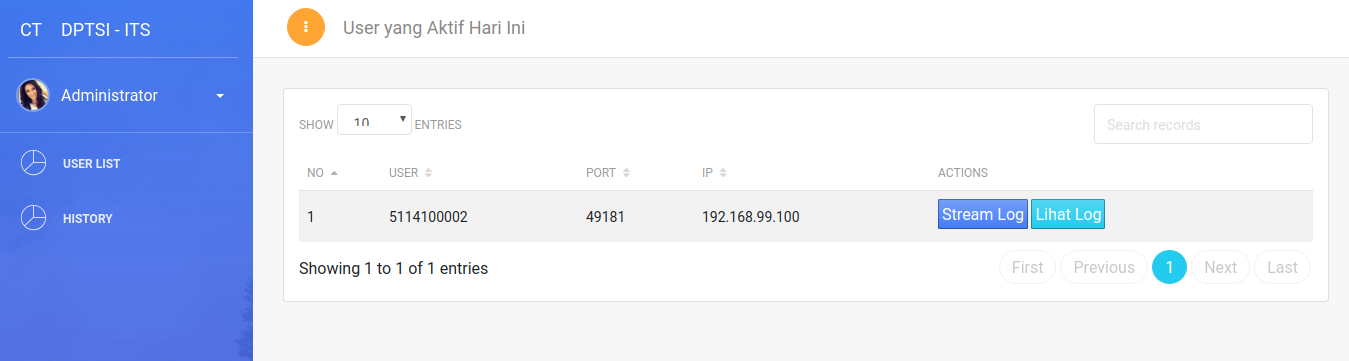
\includegraphics[width=\linewidth]{images/bab4/useraktif}
	\caption{Halaman \textit{Administrator} Menu \textit{User List}}
	\label{halamandashboardadmin}
\end{figure}

Pada bagian \textit{sidebar} terdapat dua menu yaitu \textit{User List} dan \textit{History}. Menu \textit{User List} berguna untuk melihat \textit{client} yang telah berhasil \textit{login} ke dalam sistem. Sedangkan menu \textit{history} berguna untuk melihat rekap \textit{client} yang telah berhasil \textit{login} dan mengakses internet pada hari-hari sebelumnya. Implementasi antarmuka halaman \textit{administrator} pada menu \textit{User List} dapat dilihat pada Gambar \ref{halamandashboardadmin}. Dan implementasi antarmuka halaman \textit{administrator} oada nenu \textit{History} dapat dilihat pada Gambar \ref{userrekap}

\begin{figure}[H]
	\centering
	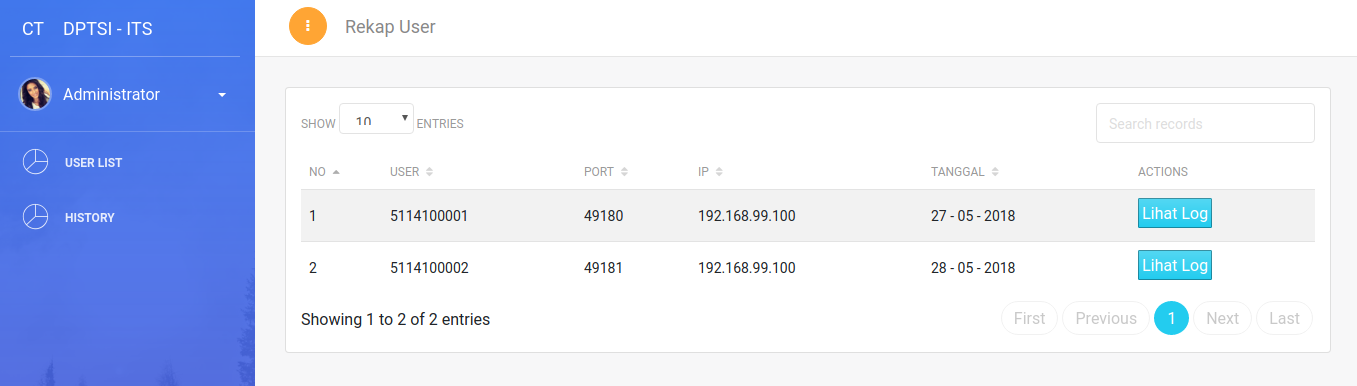
\includegraphics[width=\linewidth]{images/bab4/userrekap}
	\caption{Halaman \textit{Administrator} Menu \textit{History}}
	\label{userrekap}
\end{figure}
	\chapter{PENGUJIAN DAN EVALUASI}
	Pada bab ini akan dibahas uji coba dan evaluasi dari sistem yang telah dibuat. Sistem akan diuji coba fungsionalitas dan performanya dengan menjalankan skenario uji coba yang sudah ditentukan. Uji coba dilakukan untuk mengetahui hasil dari sistem ini sehingga dapat menjawab rumusan masalah pada tugas akhir ini.    
	
\section{Lingkungan Uji Coba}
	Lingkungan pengujian menggunakan komponen-komponen yang terdiri dari: satu \textit{server docker host}, satu \textit{server login}, dan tiga komputer penguji.Semua komputer penguji menggunakan enam buah desktop dengan sistem operasi Ubuntu 16.04
	. Pengujian dilakukan di Laboratoriom Arsitektur dan Jaringan Komputer Jurusan Teknik Informatika ITS. \\
    \indent Spesifikasi untuk setiap komponen yang digunakan ditunjukkan pada Tabel \ref{spesifikasidockerhost} untuk \textit{docker host}, Tabel \ref{spesifikasihalamanlogin} untuk \textit{server} halaman login, Tabel \ref{spesifikasikomputerpenguji1} untuk Komputer Penguji 1, Tabel \ref{spesifikasikomputerpenguji2} untuk Komputer Penguji 2, Tabel \ref{spesifikasikomputerpenguji3} untuk Komputer Penguji 3, Tabel \ref{spesifikasikomputerpenguji4} untuk Komputer Penguji 4, Tabel \ref{spesifikasikomputerpenguji5} untuk Komputer Penguji 5, dan Tabel \ref{spesifikasikomputerpenguji6} untuk Komputer Penguji 6.

\begin{enumerate}
	\item \textbf{\textit{Server} Untuk \textit{Docker Host}}
	\begin{longtable}{|l|l|}
		\caption{\textit{Server} Untuk \textit{Docker Host}}
		\label{spesifikasidockerhost} \\
		\hline
		\textbf{Perangkat Keras}      & \begin{tabular}[c]{@{}l@{}} Processor Intel(R) Core(TM) \\ i5-2120 CPU @ 3.30GHz\end{tabular} \\ \cline{2-2} 
		& RAM 8GB	\\ \cline{2-2} 
		& Hard disk 500GB \\ \hline
		\textbf{Perangkat Lunak}      & Linux Mint 18.03 64 bit \\ \cline{2-2} 
		& Docker-CE versi 1.13.1. \\ \cline{2-2} 
		& MySQL versi 5.7.18. \\ \cline{2-2} 
		& Iptables versi 1.6. \\ \cline{2-2} 
		& Python versi 3.5.2. \\ \cline{2-2} 
		& Flask versi 1.0.2.\\ \hline
		\textbf{Konfigurasi Jaringan} & IP address : 10.151.36.134 \\ \cline{2-2} 
		& Netmask : 255.255.255.0 \\ \cline{2-2} 
		& Gateway : 10.151.36.1 \\ \cline{2-2} 
		& Hostname : X450LD \\ \hline
	\end{longtable}
	
	\item \textbf{\textit{Server} Untuk Halaman Login}
	\begin{longtable}{|l|l|}
		\caption{\textit{Server} Untuk Halaman Login}
		\label{spesifikasihalamanlogin} \\
		\hline
		\textbf{Perangkat Keras}      & \begin{tabular}[c]{@{}l@{}} Processor Intel(R) Core(TM)2Duo \\ CPU E7200 @ 2.53GHz\end{tabular} \\ \cline{2-2} 
		& RAM 1GB	\\ \cline{2-2} 
		& Hard disk 20GB \\ \hline
		\textbf{Perangkat Lunak}      & Ubuntu 16.04 64 bit \\ \cline{2-2} 
		& Nginx versi 1.10.3. \\ \cline{2-2} 
		& Gunicorn versi 19.9.1. \\ \cline{2-2} 
		& Supervisor versi 3.2. \\ \cline{2-2} 
		& Python versi 3.5.2. \\ \cline{2-2} 
		& Flask versi 1.0.2.\\ \hline
		\textbf{Konfigurasi Jaringan} & IP address : 10.151.36.173 \\ \cline{2-2} 
		& Netmask : 255.255.255.0 \\ \cline{2-2} 
		& Gateway : 10.151.36.1 \\ \cline{2-2} 
		& Hostname : SERVERLOGIN \\ \hline
	\end{longtable}
	
	\item \textbf{Komputer Penguji}
	\begin{enumerate}
		\item \textbf{Komputer Penguji 1}
		\begin{longtable}{|l|l|}
			\caption{Komputer Penguji 1}
			\label{spesifikasikomputerpenguji1} \\
			\hline
			\textbf{Perangkat Keras}      & \begin{tabular}[c]{@{}l@{}} Processor Intel(R) Core(TM) \\ i5-2120 CPU @ 3.30GHz\end{tabular} \\ \cline{2-2} 
			& RAM 8GB	\\ \cline{2-2} 
			& Hard disk 500GB \\ \hline
			\textbf{Perangkat Lunak}      & Ubuntu 16.04 64 bit \\ \cline{2-2} 
			& Firefox Quantum versi 60.0.1.\\ \hline
			\textbf{Konfigurasi Jaringan} & IP address : 10.151.36.33 \\ \cline{2-2} 
			& Netmask : 255.255.255.0 \\ \cline{2-2} 
			& Gateway : 10.151.36.134 \\ \cline{2-2} 
			& Hostname : DRONA \\ \hline
		\end{longtable}
		
		\item \textbf{Komputer Penguji 2}
		\begin{longtable}{|l|l|}
			\caption{Komputer Penguji 2}
			\label{spesifikasikomputerpenguji2} \\
			\hline
			\textbf{Perangkat Keras}      & \begin{tabular}[c]{@{}l@{}} Processor Intel(R) Core(TM) \\ i3-2120 CPU @ 3.30GHz\end{tabular} \\ \cline{2-2} 
			& RAM 6GB	\\ \cline{2-2} 
			& Hard disk 1TB \\ \hline
			\textbf{Perangkat Lunak}      & Ubuntu 16.04 64 bit \\ \cline{2-2} 
			& Firefox Quantum versi 60.0.1.\\ \hline
			\textbf{Konfigurasi Jaringan} & IP address : 10.151.36.34 \\ \cline{2-2} 
			& Netmask : 255.255.255.0 \\ \cline{2-2} 
			& Gateway : 10.151.36.134 \\ \cline{2-2} 
			& Hostname : BHISMA \\ \hline
		\end{longtable}
		\pagebreak
		
		\item \textbf{Komputer Penguji 3}
		\begin{longtable}{|l|l|}
			\caption{Komputer Penguji 3}
			\label{spesifikasikomputerpenguji3} \\
			\hline
			\textbf{Perangkat Keras}      & \begin{tabular}[c]{@{}l@{}} Processor Intel(R) Core(TM) \\ i3-2120 CPU @ 3.30GHz\end{tabular} \\ \cline{2-2} 
			& RAM 4GB	\\ \cline{2-2} 
			& Hard disk 250GB \\ \hline
			\textbf{Perangkat Lunak}      & Ubuntu 16.04 64 bit \\ \cline{2-2} 
			& Firefox Quantum versi 60.0.1.\\ \hline
			\textbf{Konfigurasi Jaringan} & IP address : 10.151.36.33 \\ \cline{2-2} 
			& Netmask : 255.255.255.0 \\ \cline{2-2} 
			& Gateway : 10.151.36.134 \\ \cline{2-2} 
			& Hostname : ARJUNA \\ \hline
		\end{longtable}
		
		\item \textbf{Komputer Penguji 4}
		\begin{longtable}{|l|l|}
			\caption{Komputer Penguji 4}
			\label{spesifikasikomputerpenguji4} \\
			\hline
			\textbf{Perangkat Keras}      & \begin{tabular}[c]{@{}l@{}} Processor Intel(R) Core(TM) \\ i3-2120 CPU @ 3.30GHz\end{tabular} \\ \cline{2-2} 
			& RAM 8GB	\\ \cline{2-2} 
			& Hard disk 1TB \\ \hline
			\textbf{Perangkat Lunak}      & Ubuntu 16.04 64 bit \\ \cline{2-2} 
			& Firefox Quantum versi 60.0.1.\\ \hline
			\textbf{Konfigurasi Jaringan} & IP address : 10.151.36.38 \\ \cline{2-2} 
			& Netmask : 255.255.255.0 \\ \cline{2-2} 
			& Gateway : 10.151.36.134 \\ \cline{2-2} 
			& Hostname : KRESNA \\ \hline
		\end{longtable}
		\pagebreak
		
		\item \textbf{Komputer Penguji 5}
		\begin{longtable}{|l|l|}
			\caption{Komputer Penguji 5}
			\label{spesifikasikomputerpenguji5} \\
			\hline
			\textbf{Perangkat Keras}      & \begin{tabular}[c]{@{}l@{}} Processor Intel(R) Core(TM)2Duo \\ CPU E7200 @ 2.53GHz\end{tabular} \\ \cline{2-2} 
			& RAM 2GB	\\ \cline{2-2} 
			& Hard disk 120GB \\ \hline
			\textbf{Perangkat Lunak}      & Ubuntu 16.04 64 bit \\ \cline{2-2} 
			& Firefox Quantum versi 60.0.1.\\ \hline
			\textbf{Konfigurasi Jaringan} & IP address : 10.151.36.39 \\ \cline{2-2} 
			& Netmask : 255.255.255.0 \\ \cline{2-2} 
			& Gateway : 10.151.36.134 \\ \cline{2-2} 
			& Hostname : NARASOMA \\ \hline
		\end{longtable}
		
		\item \textbf{Komputer Penguji 6}
		\begin{longtable}{|l|l|}
			\caption{Komputer Penguji 6}
			\label{spesifikasikomputerpenguji6} \\
			\hline
			\textbf{Perangkat Keras}      & \begin{tabular}[c]{@{}l@{}} Processor Intel(R) Core(TM)2Duo \\ CPU E7200 @ 2.53GHz\end{tabular} \\ \cline{2-2} 
			& RAM 2GB	\\ \cline{2-2} 
			& Hard disk 120GB \\ \hline
			\textbf{Perangkat Lunak}      & Ubuntu 16.04 64 bit \\ \cline{2-2} 
			& Firefox Quantum versi 60.0.1.\\ \hline
			\textbf{Konfigurasi Jaringan} & IP address : 10.151.36.41 \\ \cline{2-2} 
			& Netmask : 255.255.255.0 \\ \cline{2-2} 
			& Gateway : 10.151.36.134 \\ \cline{2-2} 
			& Hostname : ANGGADA \\ \hline
		\end{longtable}
		
	\end{enumerate}
\end{enumerate}
			
			Untuk gambar arsitektur dari setiap komponen yang digunakan dapat dilihat pada Gambar \ref{arsitekturbab5}.
			
			\begin{figure}[H]
				\centering
				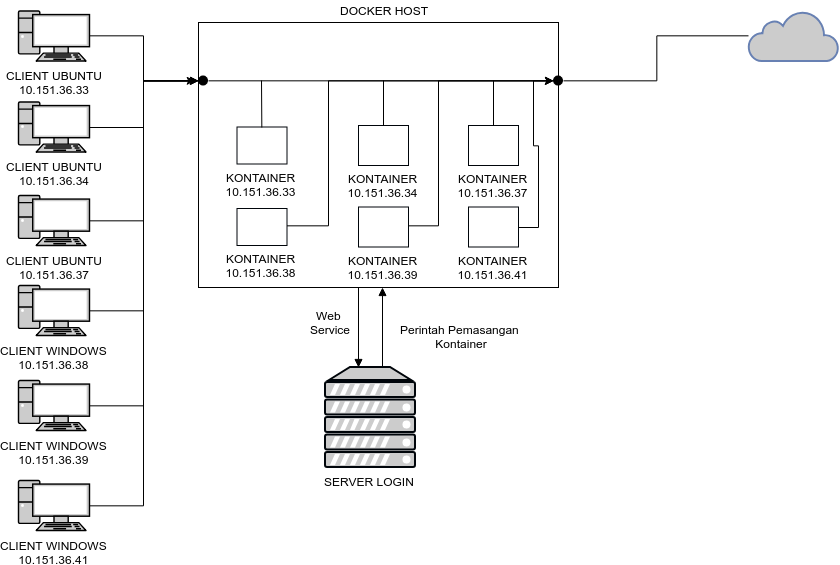
\includegraphics[width=\linewidth]{images/bab5/arsitekturbab5}
				\caption{Arsitektur dari Setiap Komponen Uji Coba}
				\label{arsitekturbab5}
			\end{figure}
			
   
\section{Skenario Uji Coba} \label{skenarioujicoba}
	Uji coba akan dilakukan untuk mengetahui keberhasilan sistem yang telah dibangun. Skenario pengujian dibedakan menjadi 2 bagian, yaitu:
    \begin{itemize}
    \item \textbf{Uji Fungsionalitas} \\
    	Pengujian ini didasarkan pada fungsionalitas yang disajikan sistem.
    \item \textbf{Uji Performa} \\
    	Pengujian ini untuk menguji ketahanan sistem terhadap sejumlah permintaan ke aplikasi secara bersamaan. Pengujian dilakukan dengan melakukan \textit{benchmark} pada sistem.
    \end{itemize}
    
\subsection{Skenario Uji Coba Fungsionalitas}
Uji coba fungsionalitas dilakukan dengan cara menjalankan sistem yang telah dibuat, dan melakukan pengujian terhadap fitur yang telah dibuat. Uji coba fungsionalitas akan berfungsi untuk memastikan sistem sudah memenuhi kebutuhan yang tertera pada Bab 3, yaitu meliputi:

\begin{enumerate}
\item Pengujian \textit{client} dapat mengakses internet.
\item Pengujian fungsionalitas menu aplikasi halaman administrator.
\end{enumerate}

\subsubsection{Uji \textit{client} dapat Mengakses Internet} \label{keempat}
Pengujian ini dilakukan untuk mengetahui apakah \textit{client} dapat mengakses internet atau tidak. Pada uji \textit{client} dapat mengakses internet akan dibagi lagi menjadi beberapa bagian, antara lain:
\begin{enumerate}
\item Pengujian \textit{client} dapat \textit{login} ke dalam sistem.
\item Pengujian \textit{client} dapat mengirimkan permintaan penyediaan kontainer \textit{docker} ke \textit{docker host}.
\item Pengujian \textit{docker host} dapat menerima permintaan penyediaan kontainer \textit{docker}.
\end{enumerate}

Pengujian menggunakan enam buah komputer penguji. Pengujian ini dapat dilakukan dengan membuka \textit{browser} dan membuka \textit{website} HTTP ataupun juga HTTPS. Daftar uji fungsionalitas \textit{client} dapat mengakses internet dijelaskan pada Tabel \ref{ujicoba4}.
\begin{longtable}{|p{0.05\textwidth}|p{0.38\textwidth}|p{0.39\textwidth}|}					\caption{Skenario Uji \textit{Client} dapat Mengakses Internet} \label{ujicoba4} \\
	\hline
	\textbf{No} & \textbf{Uji Coba} & \textbf{Hasil Harapan} \\ \hline
	\endfirsthead
	\caption[]{Skenario Uji Mengelola Aplikasi Berbasis Docker} \\
	\hline
	\textbf{No} & \textbf{Uji Coba} & \textbf{Hasil Harapan} \\ \hline
	\endhead
	\endfoot
	\endlastfoot
	
	1 & \textit{Client} membuka website HTTP maupun HTTPS dengan menggunakan \textit{browser}. & \textit{Client} dapat membuka website HTTP maupun HTTPS dengan menggunakan \textit{browser} yang ada.\\ \hline
\end{longtable}

\paragraph{Uji \textit{Client} dapat \textit{Login} ke Dalam Sistem} \label{pertama}
Pengujian ini dilakukan untuk mengetahui apakah \textit{client} sudah bisa \textit{login} ke dalam sistem saat \textit{client} akan mengakses internet. Pengujian menggunakan satu buah \textit{server} yang berperan sebagai \textit{server login} untuk \textit{client} dan menggunakan enam buah Komputer Penguji yang dijalankan dengan VirtualBox berperan sebagai \textit{client}. Pengujian dilakukan oleh \textit{client} dalam keadaan belum \textit{login} ke dalam sistem. Ketika \textit{client} mencoba membuka sebuah web, maka \textit{client} akan diarahkan ke \textit{server login} terlebih dahulu.

Alamat / IP \textit{address} dari \textit{server login} yang digunakan adalah \texttt{10.151.36.173}. Setelah \textit{client} diarahkan ke \textit{server login}, selanjutnya adalah \textit{client} harus memasukkan \textit{input username} dan \textit{password}. Daftar uji fungsionalitas \textit{client} dapat \textit{login} ke dalam sistem dijelaskan pada Tabel \ref{ujicoba1}

\begin{longtable}{|p{0.05\textwidth}|p{0.38\textwidth}|p{0.39\textwidth}|}					\caption{Skenario Uji \textit{Client} dapat \textit{Login} ke Dalam Sistem} \label{ujicoba1} \\
	\hline
	\textbf{No} & \textbf{Uji Coba} & \textbf{Hasil Harapan} \\ \hline
	\endfirsthead
	\caption[]{Skenario Uji Mengelola Aplikasi Berbasis Docker} \\
	\hline
	\textbf{No} & \textbf{Uji Coba} & \textbf{Hasil Harapan} \\ \hline
	\endhead
	\endfoot
	\endlastfoot
	
	1 & \textit{Client} membuka sebuah website ketika belum \textit{login} ke dalam sistem. & \textit{Traffic} dari \textit{client} akan diarahkan ke \textit{server login} dan \textit{client} dapat membuka halaman \textit{login} secara otomatis.\\ \hline
	2 & \textit{Client} melakukan \textit{login} ke \textit{server login}. & \textit{Client} berhasil melakukan \textit{login} dengan menggunakan \textit{username} dan \textit{password} yang sudah ditentukan.\\ \hline
\end{longtable}

\paragraph{Uji \textit{Client} dapat Mengirimkan Permintaan Penyediaan Kontainer \textit{Docker} ke \textit{Docker Host}} \label{kedua}
Pengujian ini dilakukan untuk memberikan perintah kepada \textit{docker host} untuk menyediakan kontainer \textit{docker} ke \textit{client} yang baru saja berhasil \textit{login} ke dalam sistem. Pengujian menggunakan satu buah \textit{server} yang berperan sebagai \textit{server login} yang akan mengirimkan permintaan penyediaan kontainer \textit{docker} ke \textit{docker host}.

Pengujian ini dapat dilakukan setelah \textit{client} berhasil memasukkan \textit{username} dan \textit{password} ke sistem, dan berhasil \textit{login} ke dalam sistem. Setelah itu sistem akan mengirimkan permintaan penyediaan kontainer \textit{docker} ke \textit{docker host}. Daftar uji fungsionalitas \textit{client} dapat mengirimkan permintaan penyediaan kontainer \textit{docker} ke \textit{docker} host dijelaskan pada Tabel \ref{ujicoba2}

\begin{longtable}{|p{0.05\textwidth}|p{0.38\textwidth}|p{0.39\textwidth}|}					\caption{Skenario Uji \textit{Client} dapat \textit{Login} Mengirimkan Permintaan Penyediaan Kontainer \textit{Docker}} \label{ujicoba2} \\
	\hline
	\textbf{No} & \textbf{Uji Coba} & \textbf{Hasil Harapan} \\ \hline
	\endfirsthead
	\caption[]{Skenario Uji Mengelola Aplikasi Berbasis Docker} \\
	\hline
	\textbf{No} & \textbf{Uji Coba} & \textbf{Hasil Harapan} \\ \hline
	\endhead
	\endfoot
	\endlastfoot
	
	1 & \textit{Client} mengirimkan permintaan penyediaan kontainer \textit{docker} kepada \textit{docker host}. & \textit{Client} berhasil mengirimkan permintaan penyediaan kontainer \textit{docker} kepada \textit{docker host}.\\ \hline
\end{longtable}

\paragraph{Uji \textit{Docker Host} dapat Menerima Permintaan Penyediaan Kontainer \textit{Docker}} \label{ketiga}
Pengujian ini dilakukan untuk menerima perintah permintaan penyediaan kontainer \textit{docker} pada \textit{docker host}. Pengujian menggunakan satu buah \textit{server} yang berperan sebagai \textit{docker host} yang akan menerima permintaan penyediaan kontainer \textit{docker}.

Alamat dari \textit{server} yang berperan sebagai \textit{docker host} adalah \texttt{10.151.36.134}. Setelah berhasil menerima permintaan penyediaan kontainer \textit{docker}, selanjutnya adalah sistem akan menuliskan \textit{username}, IP \textit{address}, dan \textit{port} dari \textit{client} yang telah mengirimkan permintaan penyediaan kontainer \textit{docker} ke basis data yang sudah tersedia.

Setelah selesai menuliskan \textit{username}, IP \textit{address}, dan \textit{port} dari \textit{client} yang telah mengirimkan permintaan penyediaan kontainer \textit{docker} ke basis data yang sudah tersedia, selanjutnya adalah membuat satu buah kontainer \textit{docker} dengan nama kontainer \texttt{[IP-Username-Port]}, dimana \texttt{IP} adalah IP \textit{address} dari \textit{client}, \texttt{Username} adalah \textit{username} ketika \textit{client} memasukkan \textit{inputan} kepada sistem saat akan \textit{login}, dan \texttt{Port} adalah sebuah \textit{port} khusus untuk \textit{client} tersebut.

Terakhir, pengujian yang dilakukan adalah membuat sebuah \textit{directory} pada \textit{docker host} yang berfungsi untuk menyimpan data \textit{log traffic} dari \textit{client}. \textit{Directory} ini akan dibuat pada \texttt{/container-data/[Tanggal]/[IP-USERNAME-PORT]}, dimana \texttt{Tanggal} akan sesuai dengan tanggal ketika \textit{client} berhasil \textit{login} ke dalam sistem, dan \texttt{[IP-USERNAME-PORT]} sesuai dengan yang sudah dituliskan pada basis data.

Daftar uji fungsionalitas \textit{docker host} dapat menerima permintaan penyediaan kontainer \textit{docker} dijelaskan pada Tabel \ref{ujicoba3}.

\begin{longtable}{|p{0.05\textwidth}|p{0.38\textwidth}|p{0.39\textwidth}|}					\caption{Skenario Uji \textit{Docker Host} dapat Menerima Permintaan Penyediaan Kontainer \textit{Docker}} \label{ujicoba3} \\
	\hline
	\textbf{No} & \textbf{Uji Coba} & \textbf{Hasil Harapan} \\ \hline
	\endfirsthead
	\caption[]{Skenario Uji Mengelola Aplikasi Berbasis Docker} \\
	\hline
	\textbf{No} & \textbf{Uji Coba} & \textbf{Hasil Harapan} \\ \hline
	\endhead
	\endfoot
	\endlastfoot
	
	1 & Sistem menerima permintaan penyediaan kontainer \textit{docker} dari \textit{client} pada \textit{docker host}. & Sistem berhasil menerima permintaan penyediaan kontainer \textit{docker} dari \textit{client} dan menuliskannya pada basis data pada \textit{docker host}.\\ \hline
	2 & Sistem membuat satu buah kontainer \textit{docker} untuk \textit{client} pada \textit{docker host}. & Sistem berhasil membuat satu buah kontainer \textit{docker} dengan nama sesuai yang ditulis pada basis data untuk \textit{client} yang berisi Mitmproxy pada \textit{docker host}.\\ \hline
	3 & Sistem membuat sebuah \textit{directory} pada \textit{docker host} sesuai dengan tanggal dan informasi dari \textit{client}. & Sistem berhasil membuat sebuah \textit{directory} pada \textit{docker host} sesuai dengan tanggal dan informasi dari \textit{client} yang sudah dituliskan pada basis data.\\ \hline
\end{longtable}

\subsubsection{Uji Fungsionalitas Menu Aplikasi Halaman \textit{Administrator}} \label{kelima}
Aplikasi halaman \textit{administrator} digunakan untuk membaca \textit{log traffic} dari \textit{client} yang sedang mengakses internet dan juga untuk melihat rekap \textit{client} yang telah menggunakan internet pada hari-hari sebelumnya. Aplikasi halaman \textit{administraotr} terdiri dari dua bagian utama, yaitu halaman \textit{user list}, dan \textit{history}. Rancangan pengujian dan hasil yang diharapkan ditunjukkan dengan Tabel \ref{ujicoba5}.

\begin{longtable}{|p{0.05\textwidth}|p{0.20\textwidth}|p{0.30\textwidth}|p{0.27\textwidth}|}
	\caption{Skenario Uji Fungsionalitas Aplikasi Halaman \textit{Administrator}} \label{ujicoba5} \\
	\hline
	\textbf{No} & \textbf{Menu} & \textbf{Uji Coba} & \textbf{Hasil Harapan} \\ \hline
	\endfirsthead
	\caption[]{Skenario Uji Fungsionalitas Aplikasi Dasbor}  \\
	\hline
	\textbf{No} & \textbf{Menu} & \textbf{Uji Coba} & \textbf{Hasil Harapan} \\ \hline
	\endhead
	\endfoot
	\endlastfoot
	1 & User List & Menampilkan halaman \textit{user list} pada web. & Halaman \textit{user list} dapat tampil pada web. \\ \cline{3-4}
	&& Melihat secara \textit{live} atau langsung \textit{log traffic} dari \textit{client}. & \textit{User} yang mempunyai akses membuka halaman \textit{administrator} dapat melihat secara \textit{live} atau langsung \textit{log traffic} dari \textit{client}. \\ \cline{3-4}
	&& Melihat \textit{log traffic} terakhir dari \textit{client}. & \textit{User} yang mempunyai akses membuka halaman \textit{administrator} dapat melihat \textit{log traffic} terakhir dari \textit{client}. \\ \hline
	2 & History & Melihat \textit{log traffic} dari \textit{client} pada hari-hari sebelumnya.  & \textit{User} yang mempunyai akses membuka halaman \textit{administrator} dapat melihat \textit{log traffic} dari \textit{client} pada hari-hari sebelumnya. \\ \hline
\end{longtable}

\subsection{Skenario Uji Coba Performa}
Uji performa dilakukan dengan menggunakan enam buah desktop yang berperan sebagai \textit{client} untuk melakukan akses ke internet secara bersama-sama. \textit{Client} akan mencoba mengakses internet dengan membuka website HTTP maupun HTTPS.

Percobaan dilakukan dengan dua skenario, yaitu mengakses website HTTP dan mengakses website HTTPS

\subsubsection{Uji Performa Penggunaan \textit{Memory}}
Pengujian dilakukan dengan menghitung penggunaan \textit{memory} yang terjadi pada \textit{docker host}. Penggunaan \textit{memory} di sini adalah penggunaan dari kontainer aplikasi yang sedang berjalan. Perhitungan dilakukan dengan mengambil nilai rata-rata penggunaan \textit{memory} dari masing-masing kontainer selama proses pengujian dilakukan.

\subsubsection{Uji Performa Kecepatan Menangani \textit{Request}}
Pengujian dilakukan dengan mengukur jumlah waktu yang diperlukan untuk menyelesaikan \textit{request} yang dilakukan oleh komputer penguji. Waktu yang diukur adalah saat \textit{client} berhasil melakukan \textit{login} ke dalam sistem sampai dengan \textit{client} selesai dibuatkan sebuah kontainer \textit{docker}.

Pengujian performa kecepatan menangani \textit{request} juga dilakukan dengan membandingkan performa kecepatan dari \textit{client} ketika \textit{client} melakukan \textit{download} maupun \textit{upload} sebuah file dengan menggunakan \textit{server} internet \textit{access management} secara konvensional dengan menggunakan \textit{server} internet \textit{access management} berbasis kontainer.

\subsubsection{Uji Performa Keberhasilan \textit{Request}}
Pengujian dilakukan dengan menghitung jumlah \textit{request} atau jumlah permintaan penyediaan kontainer \textit{docker} yang gagal dilakukan selama skenario dijalankan. Dari semua jumlah \textit{request} yang dikirimkan selama pengujian, akan didapatkan persen \textit{request} yang gagal dilakukan.
    
\section{Hasil Uji Coba dan Evaluasi}
Berikut dijelaskan hasil uji coba dan evaluasi berdasarkan skenario yang telah dijelaskan pada subbab \ref{skenarioujicoba}.
    
\subsection{Uji Fungsionalitas}
Berikut dijelaskan hasil pengujian fungsionalitas pada sistem yang dibangun.

\subsubsection{Uji \textit{Client} dapat Mengakses Internet}
Pengujian dilakukan sesuai dengan skenario yang dijelaskan pada subbab \ref{keempat} dan pada Tabel \ref{ujicoba4}. Pada hasil uji \textit{client} dapat mengakses internet akan dibagi lagi menjadi beberapa bagian, antara lain
\begin{enumerate}
\item Pengujian \textit{client} dapat \textit{login} ke dalam sistem.
\item Pengujian \textit{client} dapat mengirimkan permintaan penyediaan kontainer \textit{docker} ke \textit{docker host}.
\item Pengujian \textit{docker host} dapat menerima permintaan penyediaan kontainer \textit{docker}.
\end{enumerate}

Setelah melalui hasil uji yang telah disebutkan diatas, hasil pengujian \textit{client} dapat mengakses internet seperti tertera pada Tabel \ref{hasilujicoba5}

\begin{longtable}{|p{0.05\textwidth}|p{0.55\textwidth}|p{0.22\textwidth}|}					\caption{Hasil Uji Coba \textit{Client} dapat Mengakses Internet} \label{hasilujicoba5} \\
	\hline
	\textbf{No} & \textbf{Uji Coba} & \textbf{Hasil} \\ \hline
	\endfirsthead
	\caption[]{Hasil Uji Coba Mengelola Aplikasi Berbasis Docker} \\
	\hline
	\textbf{No} & \textbf{Uji Coba} & \textbf{Hasil} \\ \hline
	\endhead
	\endfoot
	\endlastfoot
	
	1 & \textit{Client} membuka sebuah website HTTP maupun HTTPS dengan menggunakan \textit{browser}. & OK. \\ \hline
\end{longtable}
Sesuai dengan skenario uji coba  yang diberikan pada Tabel \ref{ujicoba4}, hasil uji coba menunjukkan semua skenario berhasil ditangani.


\paragraph{Uji \textit{Client} dapat \textit{Login} ke Dalam Sistem}
Pengujian dilakukan sesuai dengan skenario yang dijelaskan pada subbab \ref{pertama} dan pada Tabel \ref{ujicoba1}. Hasil pengujian seperti tertera pada Tabel \ref{hasilujicoba1}.
        
\begin{longtable}{|p{0.05\textwidth}|p{0.55\textwidth}|p{0.22\textwidth}|}					\caption{Hasil Uji Coba \textit{Client} dapat \textit{Login} ke Dalam Sistem} \label{hasilujicoba1} \\
	\hline
	\textbf{No} & \textbf{Uji Coba} & \textbf{Hasil} \\ \hline
	\endfirsthead
	\caption[]{Hasil Uji Coba Mengelola Aplikasi Berbasis Docker} \\
	\hline
	\textbf{No} & \textbf{Uji Coba} & \textbf{Hasil} \\ \hline
	\endhead
	\endfoot
	\endlastfoot
	
    1 & \textit{Client} membuka sebuah website ketika belum \textit{login} ke dalam sistem. & OK. \\ \hline
    2 & \textit{Client} melakukan \textit{login} ke \textit{server login}. & OK. \\ \hline
\end{longtable}
Sesuai dengan skenario uji coba  yang diberikan pada Tabel \ref{ujicoba1}, hasil uji coba menunjukkan semua skenario berhasil ditangani.

\paragraph{Uji \textit{Client} dapat Mengirimkan Permintaan Penyediaan Kontainer \textit{Docker} ke \textit{Docker Host}}
Pengujian dilakukan sesuai dengan skenario yang dijelaskan pada subbab \ref{kedua} dan pada Tabel \ref{ujicoba2}. Hasil pengujian seperti tertera pada Tabel \ref{hasilujicoba2}.

\begin{longtable}{|p{0.05\textwidth}|p{0.55\textwidth}|p{0.22\textwidth}|}					\caption{Hasil Uji Coba \textit{Client} dapat Mengirimkan Permintaan Penyediaan Kontainer \textit{Docker} ke \textit{Docker Host}} \label{hasilujicoba2} \\
	\hline
	\textbf{No} & \textbf{Uji Coba} & \textbf{Hasil} \\ \hline
	\endfirsthead
	\caption[]{Hasil Uji Coba Mengelola Aplikasi Berbasis Docker} \\
	\hline
	\textbf{No} & \textbf{Uji Coba} & \textbf{Hasil} \\ \hline
	\endhead
	\endfoot
	\endlastfoot
	
	1 & \textit{Client} mengirimkan permintaan penyediaan kontainer \textit{docker} kepada \textit{docker host}. & OK. \\ \hline
\end{longtable}
Sesuai dengan skenario uji coba  yang diberikan pada Tabel \ref{ujicoba2}, hasil uji coba menunjukkan semua skenario berhasil ditangani.

\paragraph{Uji \textit{Docker Host} dapat Menerima Permintaan Penyediaan Kontainer \textit{Docker}}
Pengujian dilakukan sesuai dengan skenario yang dijelaskan pada subbab \ref{ketiga} dan pada Tabel \ref{ujicoba3}. Hasil pengujian seperti tertera pada Tabel \ref{hasilujicoba3}.

\begin{longtable}{|p{0.05\textwidth}|p{0.55\textwidth}|p{0.22\textwidth}|}					\caption{Hasil Uji Coba \textit{Docker Host} dapat Menerima Permintaan Penyediaan Kontainer \textit{Docker}} \label{hasilujicoba3} \\
	\hline
	\textbf{No} & \textbf{Uji Coba} & \textbf{Hasil} \\ \hline
	\endfirsthead
	\caption[]{Hasil Uji Coba Mengelola Aplikasi Berbasis Docker} \\
	\hline
	\textbf{No} & \textbf{Uji Coba} & \textbf{Hasil} \\ \hline
	\endhead
	\endfoot
	\endlastfoot
	
	1 & Sistem menerima permintaan penyediaan kontainer \textit{docker} dari \textit{client} pada \textit{docker host}. & OK. \\ \hline
	2 & Sistem membuat satu buah kontainer \textit{docker} untuk \textit{client} pada \textit{docker host}. & OK. \\ \hline
	3 & Sistem membuat sebuah \textit{directory} pada \textit{docker host} sesuai dengan tanggal dan informasi dari \textit{client}. & OK. \\ \hline
\end{longtable}
Sesuai dengan skenario uji coba  yang diberikan pada Tabel \ref{ujicoba3}, hasil uji coba menunjukkan semua skenario berhasil ditangani.
        
\subsubsection{Uji Fungsionalitas Menu Aplikasi Halaman \textit{Administrator}}
Pengujian dilakukan sesuai dengan skenario yang dijelaskan pada subbab \ref{kelima} dan pada Tabel \ref{ujicoba5}. Hasil pengujian seperti tertera pada Tabel \ref{hasilujicoba6}

\begin{longtable}{|p{0.05\textwidth}|p{0.20\textwidth}|p{0.30\textwidth}|p{0.27\textwidth}|}
	\caption{Hasil Uji Fungsionalitas Aplikasi Halaman \textit{Administrator}} \label{hasilujicoba6} \\
	\hline
	\textbf{No} & \textbf{Menu} & \textbf{Uji Coba} & \textbf{Hasil Harapan} \\ \hline
	\endfirsthead
	\caption[]{Hasil Uji Fungsionalitas Aplikasi Halaman \textit{Administrator}}  \\
	\hline
	\textbf{No} & \textbf{Menu} & \textbf{Uji Coba} & \textbf{Hasil} \\ \hline
	\endhead
	\endfoot
	\endlastfoot
	1 & User List & Menampilkan halaman \textit{user list} pada web. & OK. \\ \cline{3-4}
	&& Melihat secara \textit{live} atau langsung \textit{log traffic} dari \textit{client}. & OK. \\ \cline{3-4}
	&& Melihat \textit{log traffic} terakhir dari \textit{client}. & OK. \\ \hline
	2 & History & Melihat \textit{log traffic} dari \textit{client} pada hari-hari sebelumnya.  & OK. \\ \hline
\end{longtable}

Sesuai dengan skenario uji coba yang diberikan pada Tabel \ref{ujicoba5}, hasil uji coba menunjukkan semua skenario berhasil ditangani.

\subsection{Hasil Uji Performa}
Seperti yang sudah dijelaskan pada subbab \ref{skenarioujicoba} pengujian performa dilakukan dengan menggunakan enam buah \textit{desktop} yang berperan sebagai \textit{client} untuk melakukan akses ke internet secara bergantian. \textit{Client} akan mencoba mengakses internet dengan membuka \textit{website} HTTP maupun HTTPS.

\subsubsection{Penggunaan \textit{Memory}}
Pengujian dilakukan dengan menghitung penggunaan \textit{memory} yang terjadi pada \textit{docker host}. Penggunaan \textit{memory} di sini adalah penggunaan dari kontainer aplikasi yang sedang berjalan. Perhitungan dilakukan dengan mengambil nilai rata-rata penggunaan \textit{memory} dari masing-masing kontainer selama proses pengujian dilakukan.

\subsubsection{Kecepatan Menangani \textit{Request}}
Pengujian dilakukan dengan mengukur jumlah waktu yang diperlukan untuk menyelesaikan \textit{request} yang dilakukan oleh komputer penguji. Waktu yang diukur adalah saat \textit{client} berhasil melakukan \textit{login} ke dalam sistem sampai dengan \textit{client} selesai dibuatkan sebuah kontainer \textit{docker}.

Pengujian juga dilakukan dengan mengukur kecepatan unduh dan juga upload dari \textit{client}. Waktu yang diukur adalah saat \textit{client} mencoba mengunduh beberapa \textit{file} dari salah satu \textit{server}.

\subsubsection{Keberhasilan \textit{Request}}
Pengujian dilakukan dengan menghitung jumlah \textit{request} atau jumlah permintaan penyediaan kontainer \textit{docker} yang gagal dilakukan selama skenario dijalankan. Dari semua jumlah \textit{request} yang dikirimkan selama pengujian, akan didapatkan persen \textit{request} yang gagal dilakukan.

\section{Hasil Uji Coba dan Evaluasi}
Berikut dijelaskan hasil uji coba dan evaluasi berdasarkan skenario yang telah dijelaskan pada subbab \ref{skenarioujicoba}.

\subsection{Hasil Uji Performa}
Seperti yang sudah dijelaskan pada subbab \ref{skenarioujicoba} pengujian performa dilakukan dengan menggunakan enam buah desktop yang berperan sebagai \textit{client} untuk melakukan akses ke internet secara bergantian. \textit{Clint} akan mencoba mengakses internet dengan membuka website HTTP maupun HTTPS.

\subsubsection{Kecepatan Menangani \textit{Request}}
Dari hasil uji coba kecepatan menangani \textit{request}, yaitu kecepatan unduh dan \textit{upload} dari \textit{client}. Uji coba dilakukan dengan melakukan cek kecepatan pada website \texttt{http://www.speedtest.net/id}. Uji coba dilakukan dengan menggunakan satu komputer penguji sampai dengan enam komputer penguji secara bersamaan. Hasil dari uji coba menangani \textit{request} dapat dilihat pada Tabel \ref{kecepatanrequest2}.

\begin{longtable}{|p{0.2\textwidth}|p{0.25\textwidth}|p{0.25\textwidth}|p{0.2\textwidth}|}
	\caption{Kecepatan Menangai \textit{Request} Unduh dan \textit{Upload} Menggunakan Internet \textit{Access Management} Berbasis Kontainer} \label{kecepatanrequest2} \\
	\hline
	\textbf{Jumlah Client} & \textbf{Kecepatan unduh} & \textbf{Kecepatan \textit{Upload}} \\ \hline
	\endfirsthead
	\caption[]{Kecepatan Menangai \textit{Request} Unduh} \\
	\hline
	\endhead
	\endfoot
	\endlastfoot
	
	1 & $\pm$ 13,04 Mb & $\pm$ 13,62 Mb \\ \hline
	2 & $\pm$ 10,16 Mb & $\pm$ 9,27 Mb \\ \hline
	3 & $\pm$ 4,73 Mb & $\pm$ 4,47 Mb \\ \hline
	4 & $\pm$ 4,45 MB & $\pm$ 5,61 Mb \\ \hline
	5 & $\pm$ 3,93 MB & $\pm$ 4,55 Mb \\ \hline
	6 & $\pm$ 2,82 MB & $\pm$ 2,73 Mb \\ \hline
	
\end{longtable}

Hasil uji coba kecepatan menangani \textit{request} dengan menggunakan Internet \textit{Access Management} berbasis kontainer ditunjukkan dalam grafik pada Gambar \ref{grafikkecepatan1}.

\begin{figure}[H]
	\centering
	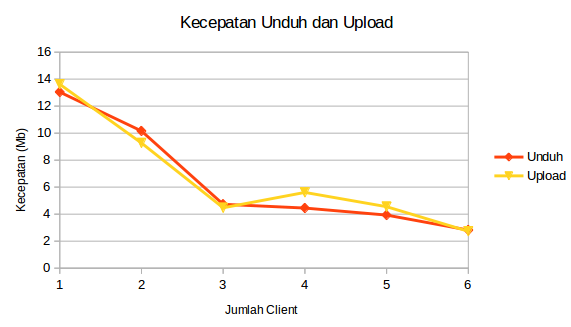
\includegraphics[width=\linewidth]{images/bab5/kecepatan1}
	\caption{Grafik Kecepatan Menangani \textit{Request}}
	\label{grafikkecepatan1}
\end{figure}

Lalu untuk uji coba dilakukan dengan enam komputer penguji dan dengan menggunakan Internet \textit{Access Management} Konvensional dapat dilihat pada Tabel \ref{kecepatanrequest3}

\begin{longtable}{|p{0.2\textwidth}|p{0.25\textwidth}|p{0.25\textwidth}|p{0.2\textwidth}|}
	\caption{Kecepatan Menangai \textit{Request} Unduh dan \textit{Upload} Menggunakan Internet \textit{Access Management} Konvensional} \label{kecepatanrequest3} \\
	\hline
	\textbf{Jumlah Client} & \textbf{Kecepatan unduh} & \textbf{Kecepatan \textit{Upload}} \\ \hline
	\endfirsthead
	\caption[]{Kecepatan Menangai \textit{Request} Unduh} \\
	\hline
	\endhead
	\endfoot
	\endlastfoot
	
	1 & $\pm$ 91,58 Mb & $\pm$ 91,27 Mb \\ \hline
	2 & $\pm$ 47,97 Mb & $\pm$ 51,49 Mb \\ \hline
	3 & $\pm$ 36,11 Mb & $\pm$ 35,28 Mb \\ \hline
	4 & $\pm$ 23,09 MB & $\pm$ 29,88 Mb \\ \hline
	5 & $\pm$ 22,50 MB & $\pm$ 26,20 Mb \\ \hline
	6 & $\pm$ 19,70 MB & $\pm$ 21,12 Mb \\ \hline
	
\end{longtable}

Hasil uji coba kecepatan menangani \textit{request} dengan menggunakan Internet \textit{Access Management} konvensional ditunjukkan dalam grafik pada Gambar \ref{grafikkecepatan2}.

\begin{figure}[H]
	\centering
	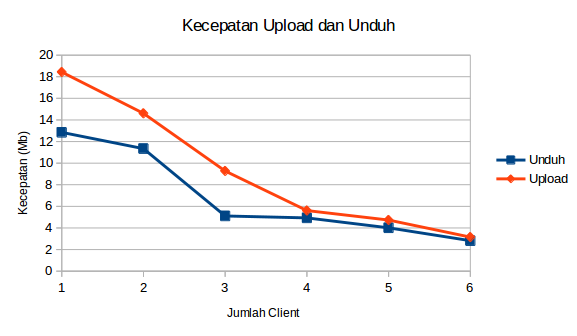
\includegraphics[width=\linewidth]{images/bab5/kecepatan2}
	\caption{Grafik Kecepatan Menangani \textit{Request}}
	\label{grafikkecepatan2}
\end{figure}

Dari Tabel \ref{kecepatanrequest2} dan Tabel \ref{kecepatanrequest3} dapat dilihat bahwa semakin banyak jumlah \textit{client}, maka semakin berkurang kecepatan unduh maupun \textit{upload} dari masing-masing \textit{client}. Hal tersebut dikarenakan \textit{bandwith} dari \textit{server} yang digunakan sebagai \textit{docker host} juga terbatas. Jika semakin besar bandwith yang dapat diterima oleh \textit{server} yang akan digunakan sebagai \textit{docker host}, maka semakin cepat pula kecepatan unduh maupun \textit{upload} dari masing-masing \textit{client}. 

\subsubsection{Penggunaan \textit{Memory}}
Dari hasil uji coba penggunaan \textit{memory}, semakin banyak \textit{request} yang diterima, semakin banyak \textit{memory} ynag diperlukan. Perhitungan penggunaan \textit{memory} adalah jumlah penggunaan dari masing-masing kontainer \textit{docker} dari \textit{client}. Dari hasil uji coba ini, dapat dilihat pada Tabel \ref{penggunaanmemory1}.

\begin{longtable}{|p{0.2\textwidth}|p{0.3\textwidth}|}
	\caption{\textit{Penggunaan \textit{Memory}}} \label{penggunaanmemory1} \\
	\hline
	\textbf{Jumlah \textit{Client}} & \textbf{Jumlah \textit{Memory} yang Digunakan} \\ \hline
	\endfirsthead

	\endhead
	\endfoot
	\endlastfoot
	
	1 & 145 MB \\ \hline
	2 & 213 MB \\ \hline
	3 & 254 MB \\ \hline
	4 & 421 MB \\ \hline
	5 & 571 MB \\ \hline
	6 & 786 MB \\ \hline
\end{longtable}
Dari Tabel \ref{penggunaanmemory1} dapat dilihat bahwa semakin banyak jumlah \textit{client} yang menggunakan Internet \textit{Access Management} berbasis kontainer, maka semakin meningkat pula penggunaan \textit{memory} dari \textit{server} yang digunakan sebagai \textit{docker host}. Rata-rata penggunaan \textit{memory} dari tiap kontainer \textit{docker} adalah sebesar $\pm$ 131 MB. Semakin besar jumlah \textit{memory} yang ada di \textit{docker host}, maka semakin banyak pula jumlah \textit{client} yang dapat ditampung.

Penggunaan \textit{memory} dari tiap kontainer juga dapat dibatasi oleh sistem jika \textit{docker host} yang digunakan hanya mempunyai \textit{memory} yang tidak terlalu besar. Hasil uji coba penggunaan \textit{memroy} ditunjukkan dalam grafik pada Gambar \ref{ram1}.

\begin{figure}[H]
	\centering
	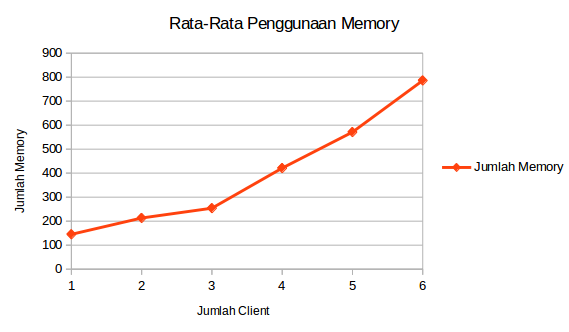
\includegraphics[width=\linewidth]{images/bab5/ram1}
	\caption{Grafik Penggunaan \textit{Memory}}
	\label{ram1}
\end{figure}

\subsubsection{Keberhasilan \textit{Request}}
Pada uji coba ini, dilakukan perhitungan seberapa besar jumlah \textit{request} yang berhasil dilakukan. Untuk jumlah \textit{client}, dapat dilihat pada Tabel \ref{keberhasilanrequest1}.

\begin{longtable}{|p{0.3\textwidth}|p{0.3\textwidth}|}
	\caption{\textit{Success Ratio Request}} \label{keberhasilanrequest1} \\
	\hline
	\textbf{\textit{Client}} & \textbf{Persen Sukses} \\ \hline
	\endfirsthead
	\caption[]{\textit{Success Ratio Request}} \\
	\hline
	\textbf{\textit{Client}} & \textbf{Persen Sukses} \\ \hline
	\endhead
	\endfoot
	\endlastfoot
	
	\textit{Client} 1 & 100\% \\ \hline
	\textit{Client} 2 & 100\% \\ \hline
	\textit{Client} 3 & 100\% \\ \hline
	\textit{Client} 4 & 100\% \\ \hline
	\textit{Client} 5 & 100\% \\ \hline
	\textit{Client} 6 & 100\% \\ \hline
\end{longtable}
Dari Tabel \ref{keberhasilanrequest1} dapat dilihat bahwa semua \textit{request} dari \textit{client} sukses dijalankan dan tidak ada \textit{error} sama sekali. Hasil uji coba tersebut berdasarkan keberhasilan \textit{client} untuk mengakses internet, mulai dari \textit{client} login ke dalam sistem sampai dengan sistem menyediakan sebuah kontainer \textit{docker} untuk \textit{client tersebut} dan berdasarkan keberhasilan \textit{client} untuk mengakses website HTTP maupun HTTPS.
	\chapter{PENUTUP}
    Bab ini membahas kesimpulan yang dapat diambil dari tujuan pembuatan sistem dan hubungannya dengan hasil uji coba dan evaluasi yang telah dilakukan. Selain itu, terdapat beberapa saran yang bisa dijadikan acuan untuk melakukan pengembangan dan penelitian lebih lanjut.
        
\section{Kesimpulan}
Dari proses perancangan, implementasi dan pengujian terhadap sistem, dapat diambil beberapa kesimpulan berikut:
\begin{enumerate}
\item Sistem dapat mengarahkan \textit{client} ke halaman \textit{login} dari sistem.
\item Sistem dapat membuatkan kontainer \textit{docker} yang berisi \textit{mitmproxy} secara otomatis ketika terdapat \textit{client} yang berhasil \textit{login} ke dalam sistem.
\item Sistem dapat mengarahkan \textit{traffic} dari \textit{client} ke kontainer \textit{docker} yang sudah dibuat dan digunakan sebagai internet \textit{access management} bagi \textit{client} dan memperbolehkan atau mengijinkan \textit{client} tersebut untuk mengakses internet. 
\end{enumerate}

\section{Saran}
Berikut beberapa saran yang diberikan untuk pengembangan lebih lanjut:
\begin{enumerate}
\item Sistem dapat dikembangkan dengan menggunakan \textit{server} lebih dari satu untuk meringankan beban kerja dari \textit{server} itu sendiri.
\item Sistem dapat dikembangkan dengan menentukan beban dari setiap \textit{server}, dengan menambahkan kriteria-kriteria yang sesuai dengan lingkungan sistem yang ada, seperti jarak antara \textit{docker host} dengan \textit{middleware} atau kecepatan bandwith dari setiap \textit{docker host} merupakan kriteria yang baik. 
\end{enumerate}

	\bibliography{Zotero}
	\bibliographystyle{IEEEtranID.bst}
    
    \renewcommand\chaptername{LAMPIRAN}
	\appendix
    \chapter{INSTALASI PERANGKAT LUNAK}

\section*{Instalasi Lingkungan Docker}
	Proses pemasangan Docker dpat dilakukan sesuai tahap berikut:
    \begin{itemize}
    \item Menambahkan repository Docker\\
    	Langkah ini dilakukan untuk menambahkan \textit{repository} Docker ke dalam paket \texttt{apt} agar dapat di unduh oleh Ubuntu. Untuk melakukannya, jalankan perintah berikut:
		\begin{tabbing}
          \texttt{sudo apt-get -y install \char`\\} \\
          \hspace{5 mm} \texttt{apt-transport-https \char`\\} \\
          \hspace{5 mm} \texttt{ca-certificates \char`\\} \\
          \hspace{5 mm} \texttt{curl} \\
          \\
          \texttt{curl -fsSL https://download.docker.com/linux/} \\
          \hspace{7 mm} \texttt{ubuntu/gpg | sudo apt-key add -} \\
          \\
          \texttt{sudo add-apt-repository \char`\\} \\
          \hspace{7 mm} \texttt{"deb [arch=amd64] https://download.docker.com/} \\
          \hspace{9 mm} \texttt{linux/ubuntu \char`\\} \\
          \hspace{7 mm} \texttt{\$ (lsb\_release -cs) \char`\\} \\
          \hspace{7 mm} \texttt{stable"} \\
          \\
          \texttt{sudo apt-get update} \\
        \end{tabbing}
        
    \item Mengunduh Docker \\
    	Docker dikembangkan dalam dua versi, yaitu CE (\textit{Community Edition}) dan EE (\textit{Enterprise Edition}). Dalam pengembangan sistem ini, digunakan Docker CE karena merupakan versi Docker yang gratis. Untuk mengunduh Docker CE, jalankan perintah \texttt{sudo apt-get -y install docker-ce}.
    
    \item Mencoba menjalankan Docker \\
    	Untuk melakukan tes apakah Docker sudah terpasang dengan benar, gunakan perintah \texttt{sudo docker run hello-world}.
    \end{itemize}

\section*{Instalasi Docker Registry} \label{install:dockerRegistry}
	Docker Registry dikembangkan menggunakan Docker Compose. Dengan menggunakan Docker Compose, proses pemasangan Docker Registry menjadi lebih mudah dan fleksibel untuk dikembangkan ditempat lain. Docker Registry akan dijalankan pada satu \textit{container} dan Nginx juga akan dijalankan di satu \textit{container} lain yang berfungsi sebagai perantara komunikasi antara Docker Registry dengna dunia luar. Berikut adalah proses pengembangan Docker Registry yang penulis lakukan:
    \begin{itemize}
    \item Pemasangan Docker Compose\\
    \$ \texttt{sudo apt-get -y install python-pip} \\
    \$ \texttt{sudo pip install docker-compose}
    
    \item Pemasangan paket \texttt{apache2-utils}\\
    	Pada paket \texttt{apache2-utils} terdapat fungsi \texttt{htpasswd} yang digunakan untuk membuat \textit{hash password} untuk Nginx. Proses pemasangan paket dapat dilakukan dengan menjalankan perintah \texttt{sudo apt-get -y install apache2-utils}.
        
    \item Pemasangan dan pengaturan Docker Registry\\
    	Buat folder \texttt{docker-registry} dan \texttt{data} dengan menjalankan perintah berikut:\\
        \$ \texttt{mkdir ~/docker-registry \&\& cd \$\_} \\
        \$ \texttt{mkdir data} \\
        Folder \texttt{data} digunakan untuk menyimpan data yang dihasilkan dan digunakan oleh \textit{container} Docker Registry. Kemudian di dalam folder \texttt{docker-registry} buat sebuah berkas dengan nama \texttt{docker-compose.yml} yang akan digunakan oleh Docker Compose untuk membangun aplikasi. Tambahkan isi berkasnya sesuai dengan Kode Sumber \ref{dockerCompose}.
        
        \begin{lstlisting}[frame=single,tabsize=2,breaklines,caption={Isi Berkas docker-compose.yml},label=dockerCompose, captionpos=b]
nginx:
image: "nginx:1.9"
ports:
	- 443:443
	- 80:80
links:
	- registry:registry
volumes:
	- ./nginx/:/etc/nginx/conf.d
registry:
	image: registry:2
	ports:
		- 127.0.0.1:5000:5000
	environment:
		REGISTRY_STORAGE_FILESYSTEM _ROOTDIRECTORY: /data
	volumes:
		- ./data:/data
		- ./registry/config.yml:/etc/docker/registry/config.yml
		\end{lstlisting}
	
    \item Pemasangan \textit{container} Nginx
    	Buat folder \texttt{nginx} di dalam folder \texttt{docker-registry}. Di dalam folder \texttt{nginx} buat berkas dengan nama \texttt{registry.conf} yang berfungsi sebagai berkas konfigurasi yang akan digunakan oleh Nginx. Isi berkas sesuai denga Kode Sumber \ref{registryConf}.
        \begin{lstlisting}[frame=single,tabsize=2,breaklines,caption={Isi Berkas registry.conf},label=registryConf, captionpos=b]
upstream docker-registry{
  server registry:5000;
}
server{
  listen 80;
  server_name registry.nota-no.life;
  return 301 https://$server_name$request_uri;
}
server{
  listen 443;
  server_name registry.nota-no.life;
  ssl on;
  ssl_certificate /etc/nginx/conf.d/cert.pem;
  ssl_certificate_key /etc/nginx/conf.d/privkey.pem;
  client_max_body_size 0;
  chunked_transfer_encoding on;
  location /v2/{
    if ($http_user_agent ~ "^(docker\/1\.(3|4|5(?!\.[0-9]-dev))|Go ).*$" ){
      return 404;
    }
    auth_basic "registry.localhost";
    auth_basic_user_file /etc/nginx/conf.d/registry.password;
    add_header 'Docker-Distribution-Api-Version' 'registry/2.0' always;
    proxy_pass http://docker-registry;
    proxy_set_header Host $http_host;
    proxy_set_header X-Real-IP $remote_addr;
    proxy_set_header X-Forwarded-For $proxy_add_x_forwarded_for;
    proxy_set_header X-Forwarded-Proto $scheme;
    proxy_read_timeout 900;
  }
}
		\end{lstlisting}
        
    \end{itemize}

\section*{Instalasi Pustaka Python} \label{install:pythonlibrary}
	Dalam pengembangan sistem ini, digunakan berbagai pustaka pendukung. Pustaka pendukung yang digunakan merupakan pustaka untuk bahasa pemrograman Python. Berikut adalah daftar pustaka yang digunakan dan cara pemasangannya:
    \begin{itemize}
    \item Python Dev \\
    	\$ \texttt{sudo apt-get install python-dev}
    \item Flask \\
    	\$ \texttt{sudo pip install Flask}
    \item docker-py \\
    	\$ \texttt{sudo pip install docker}
    \item MySQLd \\
    	\$ \texttt{sudo apt-get install python-mysqldb}
    \item Redis \\
    	\$ \texttt{sudo pip install redis}
    \item RQ \\
    	\$ \texttt{sudo pip install rq}
    \end{itemize}

\section*{Instalasi HAProxy} \label{install:haproxy}
	HAProxy dapat dipasang dengna mudah menggunakan \texttt{apt-get} karena perangkat lunak tersebut sudah tersedia pada \textit{repository} Ubuntu. Untuk melakukan pemasangan HAProxy, gunakan perintah \texttt{apt-get install haproxy}. \\
    \indent Setelah HAProxy diunduh, perangkat lunak tersebut belum berjalan karena belum diaktifkan. Untuk mengaktifkan \textit{service haproxy}, buka berkas di \texttt{/etc/default/harpoxy} kemudian ganti nilai \texttt{ENABLED} yang awalnya bernilai \texttt{0} menjadi \texttt{ENABLED=1}. Setelah itu service haproxy dapat dijalankan dengan menggunakan perintah \texttt{service harpoxy start}.
    \indent Untuk konfigurasi dari HAProxy nantinya akan diurus oleh \textit{confd}. \textit{confd} akan menyesuaikan konfigurasi dari HAProxy sesuai dengan kebutuhan aplikasi yang tersedia.

\section*{Instalasi etcd dan confd} \label{install:etcdconfd}
	etcd dapat di unggah dengan menjalankan perintah berikut, \texttt{curl https://github.com/coreos/etcd/releases/ download/v3.2.0-rc.0/etcd-v3.2.0-rc.0-linux- amd64.tar.gz}. Setelah proses unduh berhasil dilakukan, selanjutnya yang dilakukan adalah melakukan ekstrak berkasnya menggunakan perintah \texttt{tar -xvzf etcd-v3.2.0-rc.0- linux-amd64.tar.gz}. Berkas binary dari etcd bisa ditemukan pada folder \texttt{./bin/etcd}. Berkas inilah yang digunakan untuk menjalankan perangkat lunak etcd. Untuk menjalankannya, dapat dilakukan dengan menggunakan perintah \texttt{etcd --listen-client-urls http://0.0.0.0:5050 --advertise-client-urls http://128.199.250.137 :5050}. Perintah tersebut memungkinkan etcd diakses oleh \textit{host} lain dengan IP 128.199.250.137, yang merupakan host dari \textit{load balancer} dan confd. Setelah proses tersebut, etcd sudah siap untuk digunakan. \\
    \indent Setelah etcd siap digunakan, selanjutnya adalah memasang confd. Untuk menginstall confd gunakan rangkaian perintah berikut: \\
    \$ \texttt{mkdir -p \$GOPATH/src/github.com/kelseyhightower} \\
	\$ \texttt{git clone https://github.com/kelseyhightower/ confd.git \$GOPATH/src/github.com/kelseyhightower/ confd} \\
	\$ \texttt{cd \$GOPATH/src/github.com/kelseyhightower/confd} \\
	\$ \texttt{./build}
	
	Setelah berhasil memasang confd, selanjutnya buka berkas \texttt{/etc/confd/confd.toml} dan isi berkas sesuai dengan Kode Sumber \ref{confdToml}. Pengaturan tersebut bertujuan agar confd melakukan \textit{listen} terhadap server etcd dan melakukan tindakan jika terjadi perubahan pada etcd.
	\begin{lstlisting}[frame=single,tabsize=2,breaklines,caption={Isi Berkas confd.toml},label=confdToml, captionpos=b]
confdir = "/etc/confd"
interval = 20
backend = "etcd"
nodes = [
        "http://128.199.250.137:5050"
]
prefix = "/"
scheme = "http"
verbose = true
		\end{lstlisting}
	Setelah melakukan konfigurasi confd, selanjutnya adalah membuat \textit{template} konfigurasi untuk HAProxy. Buka berkas di \texttt{/etc/confd/templates/haproxy.cfg.tmpl}. Jika berkas tidak ada maka buat berkasnya dan isi berkas sesuai dengan Kode Sumber \ref{haproxyCfgTmpl}.
        
    \begin{lstlisting}[frame=single,tabsize=2,breaklines,caption={Isi Berkas haproxy.cfg.tmpl},label=haproxyCfgTmpl, captionpos=b]
global
        log /dev/log    local0
        log /dev/log    local1 notice
        chroot /var/lib/haproxy
        stats socket /run/haproxy/admin.sock mode 660 level admin
        stats timeout 30s
        daemon
defaults
        log     global
        mode    http
        option  httplog
        option  dontlognull
        timeout connect 5000
        timeout client  50000
        timeout server  50000
        errorfile 400 /etc/haproxy/errors/400.http
        errorfile 403 /etc/haproxy/errors/403.http
        errorfile 408 /etc/haproxy/errors/408.http
        errorfile 500 /etc/haproxy/errors/500.http
        errorfile 502 /etc/haproxy/errors/502.http
        errorfile 503 /etc/haproxy/errors/503.http
        errorfile 504 /etc/haproxy/errors/504.http
frontend http-in
        bind *:80

        # Define hosts
        {{range gets "/images/*"}}
        {{$data := json .Value}}
                acl host_{{$data.image_name}} hdr(host) -i {{$data.domain}}.nota-no.life
        {{end}}

        ## Figure out which one to use
        {{range gets "/images/*"}}
        {{$data := json .Value}}
                use_backend {{$data.image_name}}_cluster if host_{{$data.image_name}}
        {{end}}
{{range gets "/images/*"}}
{{$data := json .Value}}
backend {{$data.image_name}}_cluster
        mode http
        balance roundrobin
        option forwardfor
        cookie JSESSIONID prefix
        {{range $data.containers}}
        server {{.name}} {{.ip}}:{{.port}} check
        {{end}}
{{end}}
		\end{lstlisting}    

	Langkah terakhir adalah membuat berkas konfigurasi untuk HAProxy di \texttt{/etc/confd/conf.d/haproxy.toml}. Jika berkas tidak ada, maka buat berkasnya dan isi berkas sesuai dengan Kode Sumber \ref{haproxyToml}.
	\begin{lstlisting}[frame=single,tabsize=2,breaklines,caption={Isi Berkas haproxy.toml},label=haproxyToml, captionpos=b]
[template]
src = "haproxy.cfg.tmpl"
dest = "/etc/haproxy/haproxy.cfg"
keys = [
        "/images"
]
reload_cmd = "iptables -I INPUT -p tcp --dport 80 --syn -j DROP && sleep 1 && service haproxy restart && iptables -D INPUT -p tcp --dport 80 --syn -j DROP"
	\end{lstlisting}
    
    Setelah melakukan konfigurasi, selanjutnya adalah menjalankan confd dengan menggunakan perintah \texttt{confd \&}.

\section*{Pemasangan Redis} \label{install:redis}
	Redis dapat dipasang dengan mempersiapkan kebutuhan pustaka pendukungnya. Pustaka yang digunakan adalah \texttt{build-essential} dan \texttt{tcl8.5}. Untuk melakukan pemasangannya, jalankan perintah berikut:\\
	 \$ \texttt{sudo apt-get install build-essential}\\
     \$ \texttt{sudo apt-get install tcl8.5}\\
     \indent Setelah itu unduh aplikasi Redis dengan menjalankan perintah \texttt{wget http://download.redis.io/releases/redis-stable.tar.gz}. Setelah selesai diunduh, buka file dengan perintah berikut:\\
     \$ \texttt{tar xzf redis-stable.tar.gz \&\& cd redis-stable}\\
     \indent Di dalam folder \texttt{redis-stable}, bangun Redis dari kode sumber dengan menjalankan perintah \texttt{make}. Setelah itu lakukan tes kode sumber dengan menjalankan \texttt{make test}. Setelah selesai, pasang Redis dengan menggunakan perinah \texttt{sudo make install}. Setelah selesai melakukan pemasangan, Redis dapat diaktifkan dengan menjalankan berkas bash dengan nama \texttt{install\_server.sh}.\\
     Untuk menambah pengaman pada Redis, diatur agar Redis hanya bisa dari \textit{localhost}. Untuk melakukannya, buka file \texttt{/etc/redis/6379.conf}, kemudian cari baris \texttt{bind 127.0.0.1}. Hapus komen jika sebelumnya baris tersebut dalam keadaan tidak aktif. Jika tidak ditemukan baris dengan isi tersebut, tambahkan pada akhir berkas baris tersebut.

\section*{Pemasangan kerangka kerja React}
	Pada pengembangan sistem ini, penggunaan pustaka React dibangun di atas konfigurasi Create React App. Untuk memasang Create React App, gunakan perintah \texttt{npm install -g create-react-app}. Setelah terpasang, untuk membangun aplikasinya jalankan perintah \texttt{create-react-app fe-controller}. Setelah proses tersebut, dasar dari aplikasi sudah terbangun dan siap untuk dikembangkan lebih lanjut.
    \chapter{KODE SUMBER}

\section*{Let's Encrypt Cross Signed}
\begin{lstlisting}[frame=single,tabsize=2,breaklines,caption={Let's Encrypt X3 Cross Signed.pem},label=letsencryptpem, captionpos=b]
-----BEGIN CERTIFICATE-----
MIIEkjCCA3qgAwIBAgIQCgFBQgAAAVOF c2oLheynCDANBgkqhkiG9w0BAQsFADA/
MSQwIgYDVQQKExtEaWdpdGFsIFNpZ25h dHVyZSBUcnVzdCBDby4xFzAVBgNVBAMT
DkRTVCBSb290IENBIFgzMB4XDTE2MDMx NzE2NDA0NloXDTIxMDMxNzE2NDA0Nlow
SjELMAkGA1UEBhMCVVMxFjAUBgNVBAoT DUxldCdzIEVuY3J5cHQxIzAhBgNVBAMT
GkxldCdzIEVuY3J5cHQgQXV0aG9yaXR5 IFgzMIIBIjANBgkqhkiG9w0BAQEFAAOC
AQ8AMIIBCgKCAQEAnNMM8FrlLke3cl03 g7NoYzDq1zUmGSXhvb418XCSL7e4S0EF
q6meNQhY7LEqxGiHC6PjdeTm86dicbp5 gWAf15Gan/PQeGdxyGkOlZHP/uaZ6WA8
SMx+yk13EiSdRxta67nsHjcAHJyse6cF 6s5K671B5TaYucv9bTyWaN8jKkKQDIZ0
Z8h/pZq4UmEUEz9l6YKHy9v6Dlb2honz hT+Xhq+w3Brvaw2VFn3EK6BlspkENnWA
a6xK8xuQSXgvopZPKiAlKQTGdMDQMc2P MTiVFrqoM7hD8bEfwzB/onkxEz0tNvjj
/PIzark5McWvxI0NHWQWM6r6hCm21AvA 2H3DkwIDAQABo4IBfTCCAXkwEgYDVR0T
AQH/BAgwBgEB/wIBADAOBgNVHQ8BAf8E BAMCAYYwfwYIKwYBBQUHAQEEczBxMDIG
CCsGAQUFBzABhiZodHRwOi8vaXNyZy50 cnVzdGlkLm9jc3AuaWRlbnRydXN0LmNv
bTA7BggrBgEFBQcwAoYvaHR0cDovL2Fw cHMuaWRlbnRydXN0LmNvbS9yb290cy9k
c3Ryb290Y2F4My5wN2MwHwYDVR0jBBgw FoAUxKexpHsscfrb4UuQdf/EFWCFiRAw
VAYDVR0gBE0wSzAIBgZngQwBAgEwPwYL KwYBBAGC3xMBAQEwMDAuBggrBgEFBQcC
ARYiaHR0cDovL2Nwcy5yb290LXgxLmxl dHNlbmNyeXB0Lm9yZzA8BgNVHR8ENTAz
MDGgL6AthitodHRwOi8vY3JsLmlkZW50 cnVzdC5jb20vRFNUUk9PVENBWDNDUkwu
Y3JsMB0GA1UdDgQWBBSoSmpjBH3duubR ObemRWXv86jsoTANBgkqhkiG9w0BAQsF
AAOCAQEA3TPXEfNjWDjdGBX7CVW+dla5 cEilaUcne8IkCJLxWh9KEik3JHRRHGJo
uM2VcGfl96S8TihRzZvoroed6ti6WqEB mtzw3Wodatg+VyOeph4EYpr/1wXKtx8/
wApIvJSwtmVi4MFU5aMqrSDE6ea73Mj2 tcMyo5jMd6jmeWUHK8so/joWUoHOUgwu
X4Po1QYz+3dszkDqMp4fklxBwXRsW10K XzPMTZ+sOPAveyxindmjkW8lGy+QsRlG
PfZ+G6Z6h7mjem0Y+iWlkYcV4PIWL1iw Bi8saCbGS5jN2p8M+X+Q7UNKEkROb3N6
KOqkqm57TH2H3eDJAkSnh6/DNFu0Qg==
-----END CERTIFICATE-----
	\end{lstlisting}


	\appendix

	\backmatter % Lampiran tanpa judul LAMPIRAN X, biasanya untuk BIODATA PENULIS
	\chapter{BIODATA PENULIS}
		\begin{wrapfigure}{l}{0.3\textwidth}
			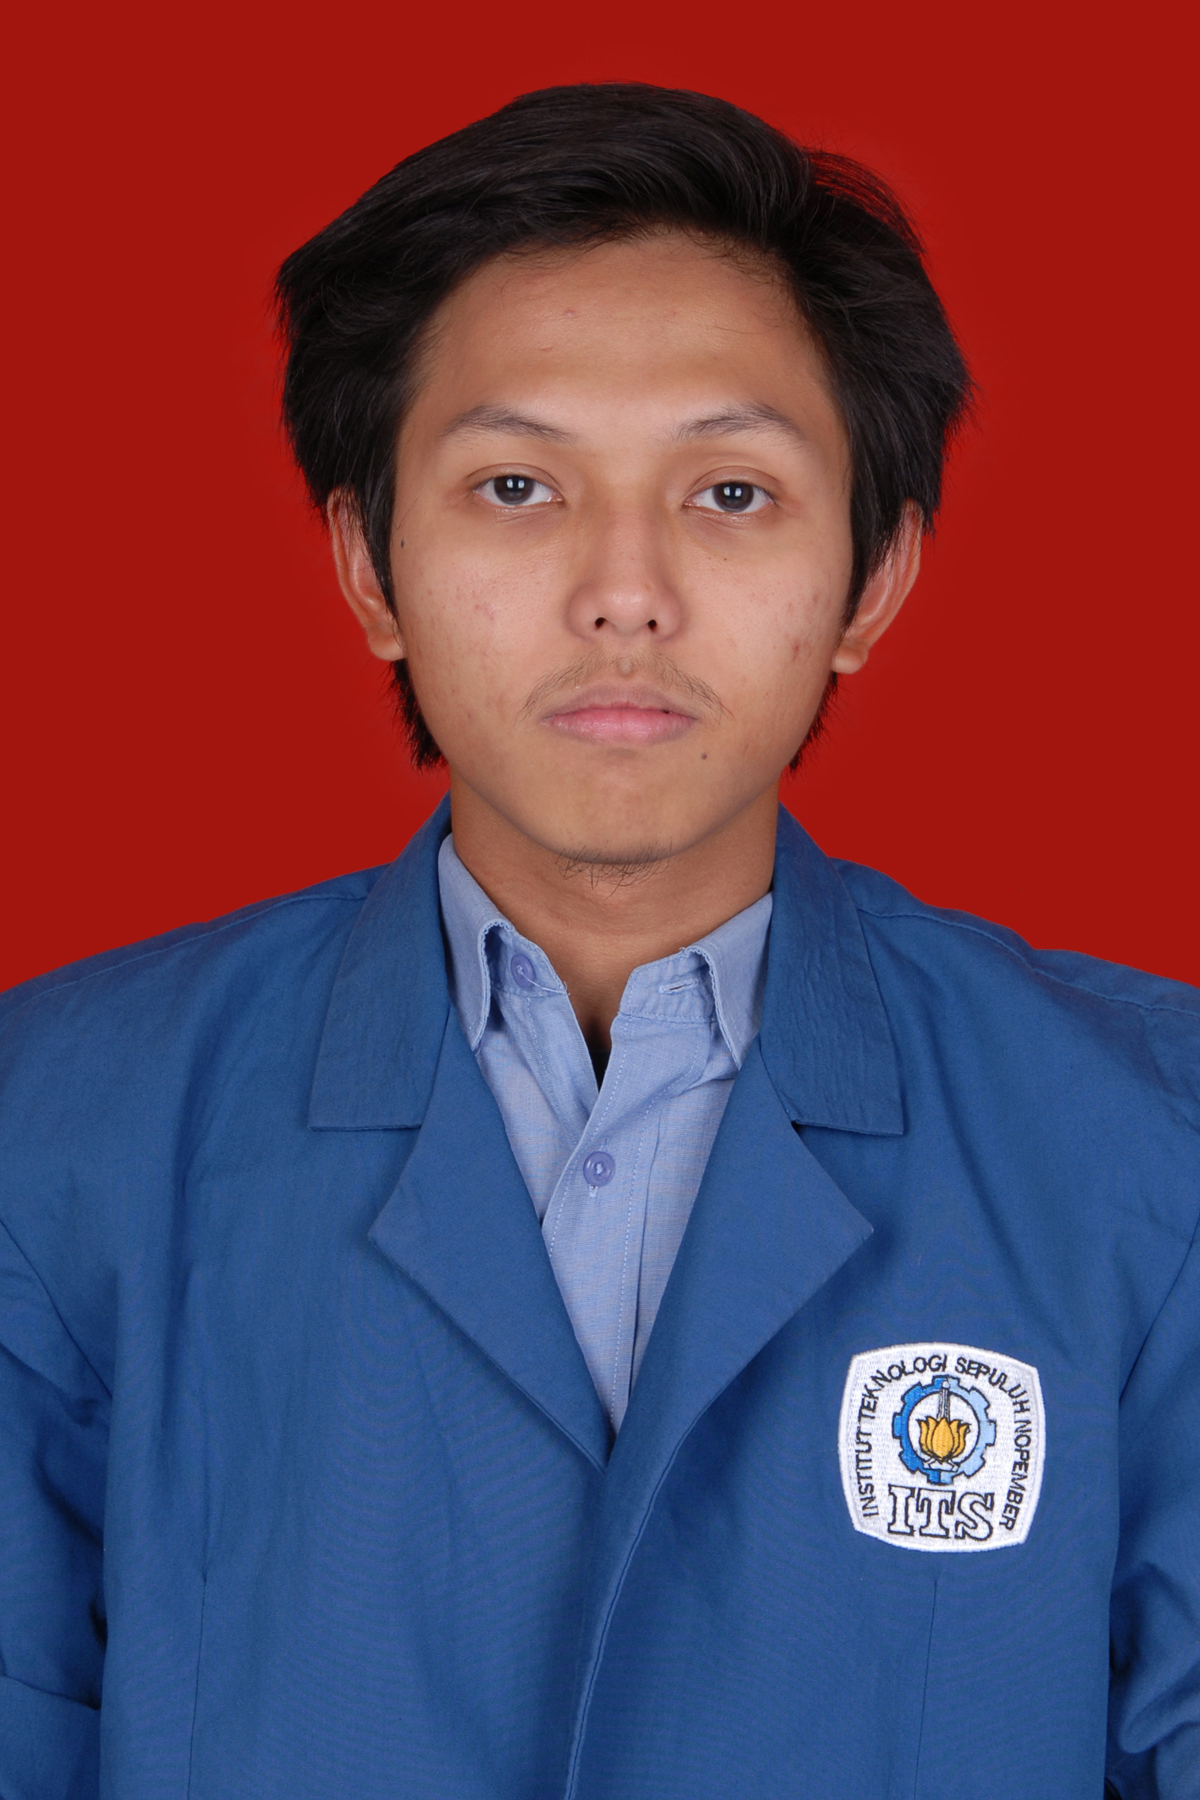
\includegraphics[width=0.29\textwidth]{images/cover/pic}
		\end{wrapfigure}
		\textbf{Fourir Akbar}, akrab dipanggil Oing, lahir pada tanggal 25 April 1996 di Surabaya. Penulis merupakan seorang mahasiswa yang sedang menempuh studi di Departemen Informatika Institut Teknologi Sepuluh Nopember. Memiliki beberapa hobi antara lain futsal dan DOTA. Pernah menjadi asisten dosen pada mata kuliah sistem operasi dan mata kuliah jaringan komputer pada semester 2016/2017 dan 2017/2018. Lalu juga pernah menjadi asisten dosen pada mata kuliah sistem terdistribusi pada tahun ajaran 2017/2018. Penulis juga pernah menjadi asisten dosen pendidikan informatika dan komputer terapan (PIKTI) ITS pada tahun ajaran 2016/2017 dan 2017/2018. Selama menempuh pendidikan di kampus, penulis juga aktif dalam organisasi kemahasiswaan, antara lain sebagai Staff Departemen Hubungan Luar Himpunan Mahasiswa Teknik Computer-Informatika pada tahun ajaran 2015/2016. Penulis juga aktif dalam kepanitiaan Schematics, antara lain sebagai Staff Biro Revolutionary Entertainment and Expo with Various Arts pada tahun ajaran 2015/2016 dan menjadi Badan Pengurus Harian (BPH) Biro Perlengkapan dan Transportasi pada tahun 2016/2017. Penulis juga merupakan salah satu administrator aktif pada Laboratorium Arsitektur dan jaringan Komputer di Departemen Informatika ITS.
\end{document}

\end{document} % YAY, WELCOME TO REAL WORD :)
